\section{A Formal Approach to Prove Compatibility}
\label{chap:compatibility:formal_approach}

\begin{copiedFrom}{SoSym MPM4CPS}

In this section, we use the definition of compatibility to derive a formal approach for proving compatibility of consistency relations.
The approach bases on two ideas:
\begin{longenumerate}
    \item A set of consistency relations in which each pair of classes is only related across one concatenation of relations is inherently compatible, because there cannot be any contradictory relations. We precisely define this in a specific notion of \emph{consistency relation trees}.
    \item A consistency relation that is redundant in a set of relations, i.e., a relation that does not alter the notion of consistency for models regarding the other relations in that set, does not affect compatibility and can thus be removed from that set of relations. % in which it is redundant.
\end{longenumerate}
Given a set of consistency relations, compatibility can be proven inductively if a consistency relation tree that is equivalent to the set of relations can be found by only removing redundant relations from that set.
Finding such an equivalent consistency relation tree serves as a \emph{witness} for compatibility of a set of relations.
In the following, we formalize and prove this inductive approach to check compatibility of a set of consistency relations.
%This constitutes our contribution \ref{contrib:formalapproach}.

The sketched approach for witnessing compatibility is based on a definition of equivalence for sets of consistency relations.
We consider two sets of consistency relations equivalent if they consider the same sets of models as consistent:

\begin{definition}[Consistency Relations Equivalence]
\label{def:equivalence}
    Let $\consistencyrelationset{CR}_{1}, \consistencyrelationset{CR}_{2}$ be two sets of consistency relations defined for a tuple of metamodels $\metamodeltuple{M}$. % = \setted{\metamodel{M}{1}, \ldots, \metamodel{M}{k}}$.
    We say that:
    \begin{align*}
        &
        \consistencyrelationset{CR}_{1} \equivalenttomath \consistencyrelationset{CR}_{2} \equivalentperdefinition \forall \modeltuple{m} \in \metamodeltupleinstanceset{M} : \\
        %& \formulaskip
        %\forall \modelset{m} = \setted{\model{m}{1}, \dots \model{m}{k}}, \model{m}{i} \in \metamodelinstances{\metamodel{M}{i}} : \\ 
        & \formulaskip%\formulaskip
        \modeltuple{m} \consistenttomath \consistencyrelationset{CR}_{1} \equivalent \modeltuple{m} \consistenttomath \consistencyrelationset{CR}_{2}
    \end{align*}
\end{definition}

%Two sets of consistency relations are considered equivalent if any set of models is either considered consistent or not by both of them in the same way.

The goal of our approach is to find a set of consistency relations that is compatible and equivalent to a given consistency relation set.
We will later use equivalence to introduce a specific notion of redundancy that is compatibility-preserving.
In the following, we first consider structures of consistency relation sets that are inherently compatible and afterwards consider redundancy as a means to find an equivalent representation of a relation set that has such a structure.

%%
%% Properties for inherent compatibility
%%
We first consider two essential properties of a consistency relation set that lead to its inherent compatibility:
\begin{properdescription}
    \item[Composability:] We show that the union of independent, compatible sets of consistency relations is compatible.
    \item[Trees:] We show that relations fulfilling a special notion of \emph{consistency relation trees} are inherently compatible.
\end{properdescription}
In consequence, we know that a consistency relation set that is composed of independent subsets of consistency relation trees is inherently compatible.
Afterwards, we discuss how to find redundant consistency relations to be able to reduce and decompose sets of relations into compositions of independent consistency relation trees.


\subsection{Independence of Consistency Relations}
\label{chap:compatibility:formal_approach:independence}

We consider consistency relation sets as independent if there are no transitive consistency relations induced by relations from both sets, i.e., for each object in a model consistency is only restricted by one of those sets.

\begin{definition}[Consistency Relation Sets Independence]
    \label{def:independence}
    Let $\consistencyrelationset{CR}_{1}$ and $\consistencyrelationset{CR}_{2}$ be two sets of consistency relations. We say that:
    \begin{align*}
        &
        \consistencyrelationset{CR}_{1} \andmath \consistencyrelationset{CR}_{2} \mathtextspacearound{are independent} \equivalentperdefinition \\
        & \formulaskip
        \forall \consistencyrelation{CR}{} \in \consistencyrelationset{CR}_{1} : \forall \consistencyrelation{CR'}{} \in \consistencyrelationset{CR}_{2} : %\\
        %& \formulaskip 
        \forall \consistencyrelation{CR}{1}, \dots, \consistencyrelation{CR}{k} \in \consistencyrelationset{CR}_{1} \cup \consistencyrelationset{CR}_{2} : \\
        & \formulaskip\formulaskip
        \consistencyrelation{CR}{} \concat \consistencyrelation{CR}{1} \concat \dots \concat \consistencyrelation{CR}{k} \concat \consistencyrelation{CR'}{} = \emptyset \\
        & \formulaskip\formulaskip
        \land \consistencyrelation{CR'}{} \concat \consistencyrelation{CR}{1} \concat \dots \concat \consistencyrelation{CR}{k} \concat \consistencyrelation{CR}{} = \emptyset
    \end{align*}
    We call $\consistencyrelationset{CR}$ \emph{connected} if there is no partition of a consistency relation set $\consistencyrelationset{CR}$ into two subsets that are independent, i.e.
    \begin{align*}
        &
        \forall \consistencyrelationset{CR}_{1}, \consistencyrelationset{CR}_{2} \subseteq \consistencyrelationset{CR} : %\\
        %& \formulaskip 
        \consistencyrelationset{CR}_{1} \cap \consistencyrelationset{CR}_{2} = \emptyset \land \consistencyrelationset{CR}_{1} \cup \consistencyrelationset{CR}_{2} = \consistencyrelationset{CR}  \\
        & \formulaskip\formulaskip
        \Rightarrow \neg (\consistencyrelationset{CR}_{1} \andmath \consistencyrelationset{CR}_{2} \mathtextspacearound{are independent)}
    \end{align*}
\end{definition}

\begin{figure}
    \centering
    \newcommand{\hdistance}{(22em+0.3*\difftoafiveimage)}
\newcommand{\vdistance}{1.5em}
\newcommand{\classwidth}{6em}

\begin{tikzpicture}

% Resident
\umlclassvarwidth{resident}{}{Resident\sameheight}{
name
}{\classwidth}

% Employee
\umlclassvarwidth[, right=\hdistance of resident.north, anchor=north]{employee}{}{Employee\sameheight}{
name
}{\classwidth}

% Location
\umlclassvarwidth[, below=\vdistance of resident.south, anchor=north]{location}{}{Location\sameheight}{
street
}{\classwidth}

% Address
\umlclassvarwidth[, below=\vdistance of employee.south, anchor=north]{address}{}{Address\sameheight}{
street
}{\classwidth}

% CONSISTENCY RELATIONS
\draw[directed consistency relation] (resident.east) -- node[pos=0, above right] {$e$} node[pos=0.5, below, align=center] {
    $\consistencyrelation{CR}{1} = \setted{ \tupled{r,e} \mid \mathvariable{e.name} = \mathvariable{r.name}}$
} node[pos=1, above left] {$r$} (employee.west);

\draw[directed consistency relation] (location.east) -- node[pos=0, above right] {$l$} node[pos=0.5, below, align=center] {
    $\consistencyrelation{CR}{2} = \setted{ \tupled{l,a} \mid \mathvariable{l.street} = \mathvariable{a.street}}$
} node[pos=1, above left] {$a$} (address.west);

\end{tikzpicture}
%    \includegraphics[width=\columnwidth]{figures/independence_example.png}
    \caption[Two independent sets of consistency relations]{Two independent (sets of) consistency relations. Taken from \owncite{klare2020compatibility-report}.}
    \label{fig:compatibility:independence_example}
\end{figure}

%We call two consistency relation sets independent if the sets of elements that they relate to each other are completely independent of each other.
\begin{example}
\autoref{fig:compatibility:independence_example} depicts a simple example with two consistency relations $\consistencyrelation{CR}{1}$ and $\consistencyrelation{CR}{2}$, each relating instances of two disjoint classes with each other.
Since there is no overlap in the objects that are related by the consistency relations, they are considered independent according to \autoref{def:independence}.
\end{example}

An important property of independent sets of consistency relations is that computing their union is compatibility-preserving, i.e., the union of compatible, independent consistency relation sets is compatible as well:

\begin{theorem}[Independent Relation Sets Compatibility] \label{theorem:independencecompatibility}
    Let $\consistencyrelationset{CR}_{1}$ and $\consistencyrelationset{CR}_{2}$ be two compatible sets of consistency relations. Then $\consistencyrelationset{CR}_{1} \cup \consistencyrelationset{CR}_{2}$ is compatible.
\end{theorem}

\todoLater{Revise proof with explicit references to independence definition}
\begin{proof}
    Since $\consistencyrelationset{CR}_{1}$ is compatible, per definition there is a model tuple $\modeltuple{m}$ for each condition element $\conditionelement{c}{}$ of the left condition of each consistency relation in $\consistencyrelationset{CR}_{1}$ that contains $\conditionelement{c}{}$ and that is consistent to $\consistencyrelationset{CR}_{1}$.
    Taking such an $\modeltuple{m}$, we create a new $\modeltuple{m'}$ by removing all elements from $\modeltuple{m}$, which are contained in any condition elements in any consistency relation in $\consistencyrelationset{CR}_{2}$ and thus potentially require other elements to occur to be considered consistent to that consistency relation.
    In consequence, $\modeltuple{m'}$ does not contain any condition elements from consistency relations in $\consistencyrelationset{CR}_{2}$ and is thus consistent to $\consistencyrelationset{CR}_{2}$ by definition. 
    Additionally, $\modeltuple{m'}$ is still consistent to $\consistencyrelationset{CR}_{1}$, because due to the independence of $\consistencyrelationset{CR}_{1}$ and $\consistencyrelationset{CR}_{2}$, there cannot be any consistency relations in $\consistencyrelationset{CR}_{1}$, which require the existence of the removed elements.
    In consequence, for each condition element $\conditionelement{c}{}$ of each consistency relation in $\consistencyrelationset{CR}_{1}$ there is a model tuple that contains $\conditionelement{c}{}$ and that is consistent to $\consistencyrelationset{CR}_{1} \cup \consistencyrelationset{CR}_{2}$.
    The analogous argumentation applies to the consistency relations in $\consistencyrelationset{CR}_{2}$, which is why the definition of compatibility is fulfilled for all condition elements of all consistency relations in $\consistencyrelationset{CR}_{1} \cup \consistencyrelationset{CR}_{2}$.
\end{proof}

The constructive proof can also be reflected exemplarily in \autoref{fig:compatibility:independence_example}: Take any tuple of models that, for example, contains a resident with an arbitrary name and is consistent to $\consistencyrelation{CR}{1}$, i.e., that also contains an employee with the same name.
If that tuple of models contains any addresses or locations, they can be removed %without removing the resident from the model and 
without violating consistency to $\consistencyrelation{CR}{1}$, because addresses and locations are independently related by $\consistencyrelation{CR}{2}$.

\todo{Actually, addresses may not be removable because they are referenced by persons. However, if such a reference always needs to be set, this is a restriction that we do not reflect yet in the metamodel formalism. On the other hand, if the reference was relevant for consistency in the first consistency relation, it would have to be considered there as well, thus address would be part of that consistency relation.}


\subsection{Consistency Relation Trees}

\mnote{Intuitively, trees are compatible}
We want to find a property or specific structure of consistency relation sets, which leads to inherent consistency of the contained relations.
If we can then prove for a set of relations that we reduce it to such a structure in a compatibility-preserving way, we know that the relations are compatible.
Intuitively, such a structure is given by a kind of trees, because then there are no two concatenations of consistency relations which can relate elements in a contradictory way.

\begin{figure}
    \centering
    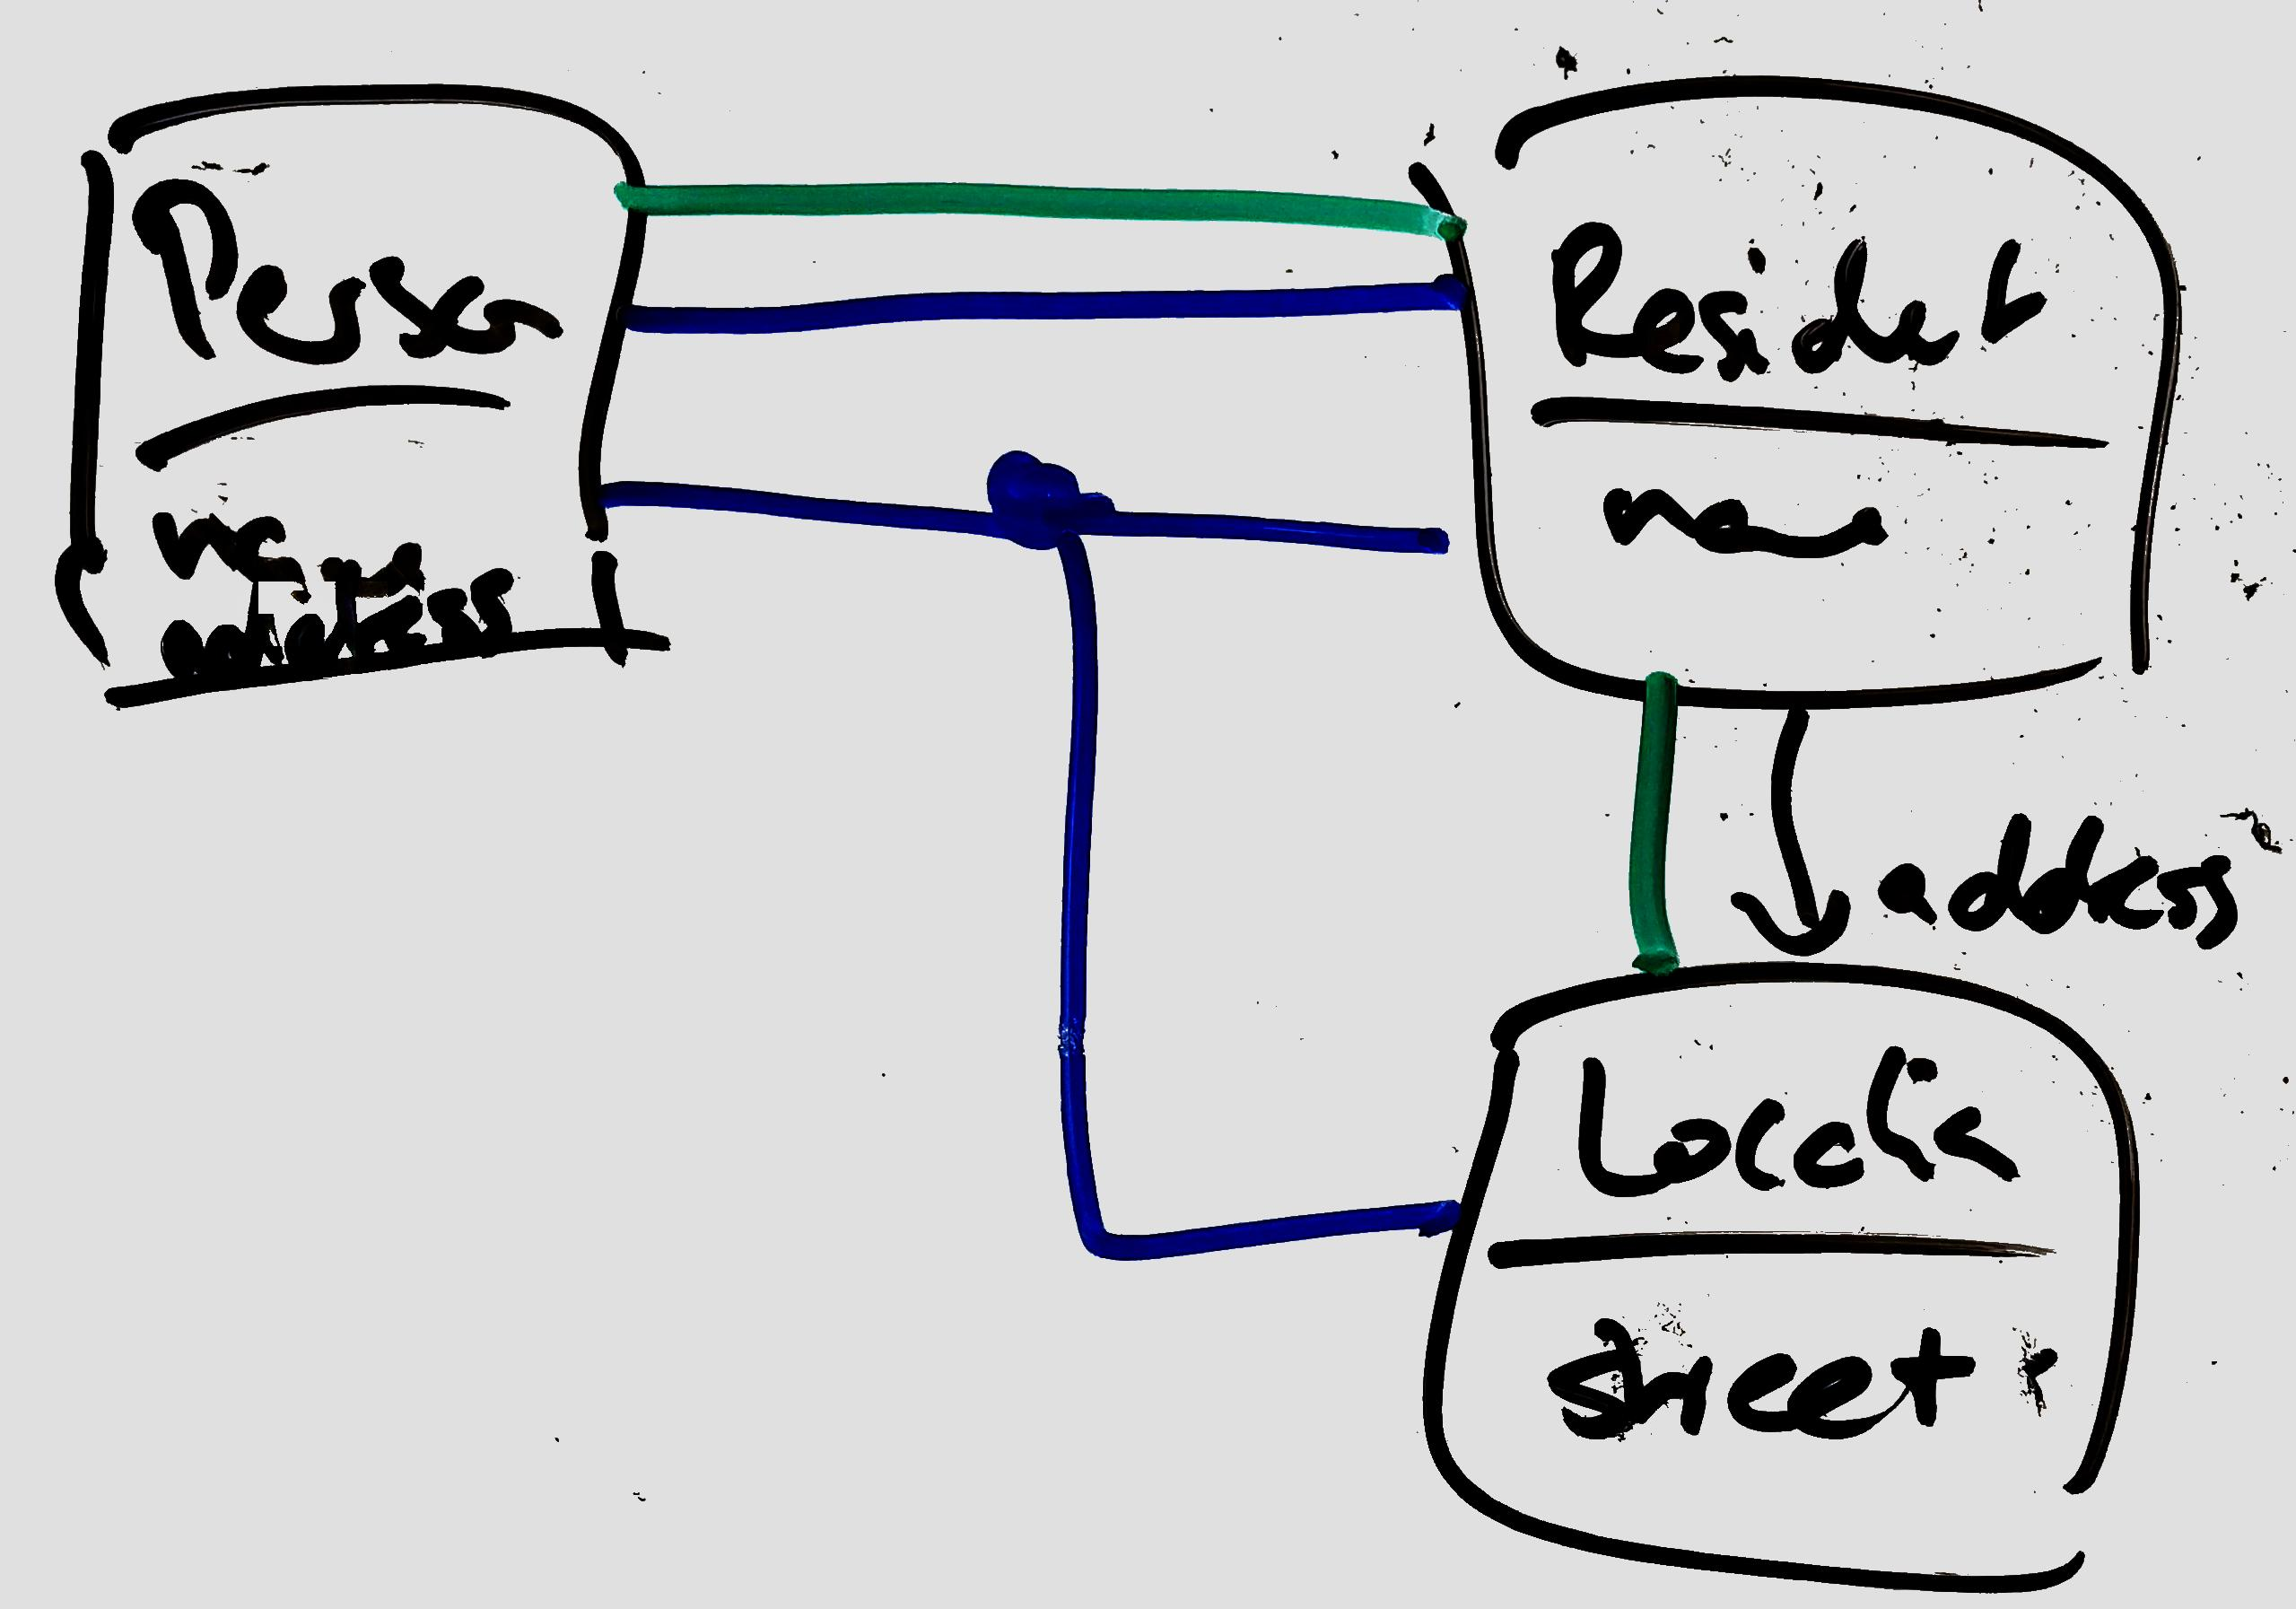
\includegraphics[width=0.5\textwidth]{figures/correctness/compatibility/hypertree.jpg}
    \caption[A hypertree with its host graph]{A hypertree (blue edges) with its host graph (green edges).}
    \label{fig:compatibility:hypertree}
\end{figure}

\mnote{Relations may be compatible if their induced hypergraphs are hypertrees}
Since consistency relations put tuple of classes into relation, it may seem natural to use a hypergraph, consisting of the classes as vertices and the class tuples of the consistency relations as hyperedges, to describe them, and expect that if the hypergraph induced by the consistency relations forms a hypertree\footnote{A hypergraph is a hypertree if there is a tree, such that every edge of the hypergraph is a set of vertices of a connected subtree of the tree~\cite{brandstaedt1998hypertrees}. Such a tree is called a \emph{host graph}.}, it is compatible.
An example for a hypertree is depicted in \autoref{fig:compatibility:hypertree}.
It consists of two hyperedges, one only relating persons and residents and one relating persons with residents and their address locations.
This is a scenario that may occur when one consistency relation puts persons and residents with their names into relation, and another describes the relation of their addresses.
These relations form a hypertree, as there is a tree, depicted in the figure, of which the vertices of all hyperedges are connected subtrees.

\mnote{Relations inducing hypertrees are not necessarily compatible}
The relations in the example may, however, not be necessarily compatible.
They can, for example, define a contradictory relation between the names of persons and residents.
In general, hypertrees induced by consistency relations are not necessarily compatible, because hyperedges can be subsets of other hyperedges and the relations inducing these hyperedges may contradict each other.
Additionally, the hyperedges to do only put sets of classes into relation and are not able distinguish between the sets belonging to different metamodels.
Thus, we have to exclude that the same classes are put into relation by multiple consistency relations in a different way.
This leads to our definition consistency relation trees.

\todoLater{Maybe we can remove symmetry and define some restriction for inverse relations. It could be useful to think about implicit relations, which are induced by another one, so that the "signatures" of forward and backward direction match.}
\begin{definition}[Consistency Relation Tree] \label{def:relationtree}
    Let $\consistencyrelationset{CR}$ be a symmetric, connected set of consistency relations. 
    %Let $\alpha = \setted{\tupled{\consistencyrelation{CR}{1}, \consistencyrelation{CR}{2}} \in \consistencyrelationset{CR} \times \consistencyrelationset{CR} \mid \classtuple{C}{r,\consistencyrelation{CR}{1}} \cap \classtuple{C}{l,\consistencyrelation{CR}{2}} \neq \emptyset \land \classtuple{C}{r,\consistencyrelation{CR}{2}} \cap \classtuple{C}{l,\consistencyrelation{CR}{1}} = \emptyset}$ be a relation on the consistency relations in $\consistencyrelationset{CR}$.
    We say:
    \begin{align*}
        &
        \consistencyrelationset{CR} \mathtextspacearound{is a consistency relation tree} \equivalentperdefinition \\
        & \formulaskip
        %\alpha \mathtext{induces a tree on} \consistencyrelationset{CR}
        \forall \consistencyrelation{CR}{} = \consistencyrelation{CR}{1} \concat \dots \concat \consistencyrelation{CR}{m}  \in \transitiveclosure{\consistencyrelationset{CR}} : \\
        & \formulaskip
        \forall \consistencyrelation{CR'}{} = \consistencyrelation{CR'}{1} \concat \dots \concat \consistencyrelation{CR'}{n} \in \transitiveclosure{\consistencyrelationset{CR}} \setminus \consistencyrelation{CR}{} : \\
        & \formulaskip\formulaskip
        \forall s, t \mid s \neq t: 
        \consistencyrelation{CR}{s} \neq \consistencyrelation{CR^T}{t} \land \consistencyrelation{CR'}{s} \neq \consistencyrelation{CR'^T}{t} \\
        & \formulaskip\formulaskip
        \Rightarrow
        \classtuple{C}{l,\consistencyrelation{CR}{}} \cap
        \classtuple{C}{l,\consistencyrelation{CR'}{}} = \emptyset
        \lor \classtuple{C}{r,\consistencyrelation{CR}{}} \cap
        \classtuple{C}{r,\consistencyrelation{CR'}{}} = \emptyset
        %
        % \forall \tupled{\consistencyrelation{CR}{1}, \dots, \consistencyrelation{CR}{k}},  \tupled{\consistencyrelation{CR'}{1}, \dots, \consistencyrelation{CR'}{m}} \in \consistencyrelationset{CR} : \\
        % & \formulaskip\formulaskip
        % \tupled{\consistencyrelation{CR}{1}, \dots, \consistencyrelation{CR}{k}} \neq \tupled{\consistencyrelation{CR'}{1}, \dots, \consistencyrelation{CR'}{m}} \\
        % & \formulaskip\formulaskip\formulaskip
        % \land \forall i, j \mid i \neq j: 
        % \consistencyrelation{CR}{i} \neq \consistencyrelation{CR^T}{j} \land \consistencyrelation{CR'}{i} \neq \consistencyrelation{CR'^T}{j} \\
        % & \formulaskip\formulaskip
        % \Rightarrow
        % \classtuple{C}{l,\consistencyrelation{CR}{1}} \cap
        % \classtuple{C}{l,\consistencyrelation{CR'}{1}} = \emptyset
        % \lor \classtuple{C}{r,\consistencyrelation{CR}{m}} \cap
        % \classtuple{C}{r,\consistencyrelation{CR'}{m}} = \emptyset
        %
        % \forall \consistencyrelation{CR}{1}, \dots, \consistencyrelation{CR}{k} \in \consistencyrelationset{CR} \mid \consistencyrelation{CR}{i} \neq \consistencyrelation{CR}{j}, \consistencyrelation{CR}{i} \neq \consistencyrelation{CR^T}{j} : \\
        % & \formulaskip\formulaskip
        % \classtuple{C}{l,\consistencyrelation{CR}{1}\concat\dots\concat\consistencyrelation{CR}{k}} \cap
        % \classtuple{C}{r,\consistencyrelation{CR}{1}\concat\dots\concat\consistencyrelation{CR}{k}} = \emptyset
        % \forall \class{C}{l} \in
        % \classtuple{C}{l,\consistencyrelation{CR}{1}\concat\dots\concat\consistencyrelation{CR}{k}} :
        % \forall \class{C}{r} \in \classtuple{C}{r,\consistencyrelation{CR}{1}\concat\dots\concat\consistencyrelation{CR}{k}}: \\
        % & \formulaskip\formulaskip
        % \class{C}{l} \cap \class{C}{r} = \emptyset
    \end{align*}
\end{definition}
\todo{We have to assume, that no element is mapped to two elements of the same class, because then it would be possible to have an incompatible network}

The definition of a consistency relation tree requires that there are no sequences of consistency relations that put the same classes into relation, i.e. between all pairs of classes there is only one concatenation of consistency relations that puts them into relation.
Since we assume a symmetric set of consistency relations, we exclude the symmetric relations from that argument, as otherwise there would always be two such concatenations by adding a consistency relation and its transposed relation to any other concatenation.

\begin{figure}
    \centering
    \newcommand{\hdistance}{14em}
\newcommand{\classwidth}{6em}

\begin{tikzpicture}

% Person
\umlclassvarwidth{person}{}{Person\sameheight}{
firstname\\
lastname
}{\classwidth}

% Employee
\umlclassvarwidth[,above right=3.5em and \hdistance of person.center, anchor=south]{employee}{}{Employee\sameheight}{
name
}{\classwidth}

\umlclassvarwidth[,right=\hdistance of person.south, anchor=south]{resident}{}{Resident\sameheight}{
name
}{\classwidth}


% CONSISTENCY RELATIONS
\draw[consistency relation] (resident.west-|person.east) -- node[pos=0, above right] {$p$} node[pos=0.5, below] {$\consistencyrelation{CR}{1}$} node[pos=1, above left] {$r$} (resident.west);
\draw[consistency relation] (resident.north) -- node[pos=0, above left] {$r$} node[right, align=left] {$\consistencyrelation{CR}{2}$} node[pos=1, below left] {$e$} (employee.south);


\node[consistency related element, below left=1em and 2em of person.south west, anchor=north west] {
$\begin{aligned}
    \consistencyrelation{CR}{1} =\; & \setted{\tupled{p,r} \mid r.name = p.firstname + "\textnormal{\textvisiblespace}" + p.lastname}\\ %[0.3em]
    \consistencyrelation{CR}{2} =\; & \setted{\tupled{r,e} \mid r.name = e.name}
\end{aligned}$
};

\end{tikzpicture}
    %\includegraphics[width=\columnwidth]{figures/tree_example.png}
    \caption[A consistency relation tree]{A consistency relation tree $\setted{\consistencyrelation{CR}{1}, \consistencyrelation{CR^T}{1}, \consistencyrelation{CR}{2}, \consistencyrelation{CR^T}{2}}$. Taken from \owncite{klare2020compatibility-report}.}
    \label{fig:compatibility:tree_example}
\end{figure}

\begin{example}
\autoref{fig:compatibility:tree_example} depicts a rather simple consistency relation tree. 
Persons are related to residents and residents are related to employees, all having the same names respectively a concatenation of $firstname$ and $lastname$, by the relations $\consistencyrelation{CR}{1}, \consistencyrelation{CR}{2}$, as well as their transposed relations $\consistencyrelation{CR^T}{1}, \consistencyrelation{CR^T}{2}$.
There are no classes that are put into relation across different paths of consistency relations, thus the definition for a consistency relation tree is fulfilled. 
If an additional relation between persons and employees was specified, like in \autoref{fig:compatibility:three_persons_example_extended}, the tree definition would not be fulfilled.
\end{example}

The definition also covers the more complicated case in which multiple classes may be put into relation by consistency relations but there is only a subset of them that is put into relation by different consistency relations.
%
%\todoDiss{Subsection with discussion about why hypertrees are not suitable here}
%
We can now prove that a set of consistency relations that is a consistency relation tree is always compatible.
To not disturb the reading flow wie the complexity of the proof for that statement, the complete proof with an auxiliary lemma can be found in \autoref{chap:appendix:compatibility_proofs}.
We only provide a proof sketch in the following.

\begin{theorem}[Consistency Relation Tree Compatibility] \label{theorem:treecompatibility}
    Let $\consistencyrelationset{CR}$ be a consistency relation tree, then $\consistencyrelationset{CR}$ is compatible.
\end{theorem}

\begin{figure}
    \centering
    \newcommand{\hdistance}{10.6em}
\newcommand{\objectwidth}{6.8em}

\begin{tikzpicture}[
    consistency process/.style={consistency execution}
]

% Person
\umlobjectvarwidth{person}{}{: Person\sameheight}{
firstname = "Alice"\\
lastname = "Avid"
}{\objectwidth-0.3em}

% Resident
\umlobjectvarwidth[,right=\hdistance-0.3em of person.center, anchor=center]{resident}{}{: Resident\sameheight}{
name = "Alice Avid"
}{\objectwidth}

% Employee
\umlobjectvarwidth[,right=\hdistance of resident.center, anchor=center]{employee}{}{: Employee\sameheight}{
name = "Alice Avid"
}{\objectwidth}


% CONSISTENCY RELATIONS
\draw[directed consistency relation] ([yshift=-1em]person.east) -- node[pos=0, above right] {$p$} node[below] {$\consistencyrelation{CR}{1}$} node[pos=1, above left] {$r$} ([yshift=-1em]resident.west);
\draw[directed consistency relation] ([yshift=-1em]resident.east) -- node[pos=0, above right] {$r$} node[below] {$\consistencyrelation{CR}{2}$} node[pos=1, above left] {$e$} ([yshift=-1em]employee.west);

\node[consistency related element, below=1.5em of resident.south, anchor=north, inner sep=0em] {
$\begin{aligned}
    \consistencyrelation{CR}{1} =\; & \setted{\tupled{p,r} \mid r.name = \mathvariable{p.firstname} + "\text{\textvisiblespace}" + \mathvariable{p.lastname}}\\[0.3em]
    \consistencyrelation{CR}{2} =\; & \setted{\tupled{r,e} \mid \mathvariable{r.name} = \mathvariable{e.name}}
\end{aligned}$
};

% CONSISTENCY PROCESS
\draw[consistency process] ([yshift=1em,xshift=-2em]person.west) -- node[above] {1.} ([yshift=1em]person.west);
\draw[consistency process] ([yshift=1em]person.east) -- node[above] {2.} ([yshift=1em]resident.west);
\draw[consistency process] ([yshift=1em]resident.east) -- node[above] {3.} ([yshift=1em]employee.west);

\end{tikzpicture}
    %\includegraphics[width=\columnwidth]{figures/tree_construction_example.png}
    \caption[Construction of a model tuple for a consistency relation tree]{An example for constructing a model with the condition element of $\consistencyrelation{CR}{1}$ containing the person named "Alice Avid" for a consistency relation tree according to the consistency relations in \autoref{fig:compatibility:tree_example}. Taken from \owncite{klare2020compatibility-report}.}
    \label{fig:compatibility:tree_construction_example}
\end{figure}

\begin{proof}[Proof Sketch]
    The complete proof is given in \autoref{chap:appendix:compatibility_proofs}.
    It is based on the proven insight that in a consistency relation tree, starting with each of the consistency relations there is a sequence of the consistency relations such that there is no overlap in the classes of the conditions at the right sides of these relations and that for each relation there is no overlap in the classes of the condition at the left side with the ones at the right side of any subsequent relation in the sequence.
    More informally speaking, the relations induce no cycle between any of the classes in the metamodels.
    We can use this insight to define a construction approach for such sequences given a set of consistency 
    relations that forms a consistency relation tree.
    For proving compatibility, we need to show that for each condition element in a consistency relation we are able to find a consistent model tuple that contains this condition element.
    Thus, starting from each condition element of each relation, we add a corresponding element according to the consistency relation.
    We then inductively add further elements for the just added elements, which are required by further consistency relations.
    Due to the defined properties of consistency relation trees, we can show that this construction is always possible and terminates with a consistent tuple of models.
    
    A simple example for that construction is depicted in \autoref{fig:compatibility:tree_construction_example}, based on the relations in the consistency relation tree in \autoref{fig:compatibility:tree_example}, and more precisely explained in the complete proof.
    The example shows the construction for the condition element with the person named \enquote{Alice Avid}, consecutively selecting consistency relations for whose fulfillment further elements, namely an appropriate resident and employee, are added.
\end{proof}

%%
%% Summary: Independent trees are compatible
%%
Summarizing, \autoref{theorem:independencecompatibility} and \autoref{theorem:treecompatibility} have shown that consistency relation sets fulfilling a special notion of trees are compatible and that combining compatible independent sets of relations is compatibility-preserving.
In consequence, having a consistency relation set that consists of independent subsets that are consistency relation trees, this set of relations is inherently compatible.
An approach that evaluates whether a given set of consistency relations fulfills \autoref{def:independence} and \autoref{def:relationtree} for independence and trees can be used to prove compatibility of those relations.

%%
%% Transition: Actual sets may generally not be trees
%%
However, consistency relations fulfill such a structure only in specific cases.
In general, like in our motivational example in \autoref{fig:compatibility:three_persons_example_extended}, there may be different consistency relations putting the same elements into relation, such that the definition for consistency relation trees is not fulfilled.
In the following, we discuss how to find a consistency relation tree that is equivalent to a given set of consistency relations, such that this equivalence witnesses compatibility.



\subsection{Redundancy of Consistency Relations}
\label{chap:compatibility:formal_approach:redundancy}

%\todoDiss{Add a definition for a \emph{compatibility-preserving consistency relation} that states that is preserved compatibility and use that for clarifying the following lemmas and theorems.}

%%
%% Problem: Not having a compatible structure, compatibility is unclear
%%
We have introduced specific structures of consistency relations that are inherently compatible.
If a given set of consistency relations does not represent one of those structures, especially because there are multiple consistency relations putting the same classes into relation, it is unclear whether such a set is compatible.

%%
%% Idea: Find and virtually remove redundant relations
%%
In the following, we present an approach to reduce a set of consistency relations to a structure of independent consistency relation trees.
The essential idea is to find relations within the set, which do not change compatibility of the consistency relation set whether or not they are contained in it.
An approach that finds such relations and---virtually---removes them from the set until the remaining relations form a set of independent consistency relation trees, proves compatibility of the given set of relations.
We first define the term of a \emph{compatibility-preserving} relation.

\begin{definition}[Compatibility-Preserving Consistency Relation]
    \label{def:compatibilitypreserving}
    Let $\consistencyrelationset{CR}$ be a compatible set of consistency relations and let $\consistencyrelation{CR}{}$ be a consistency relation. We say that:
    \begin{align*}
        &
        \consistencyrelation{CR}{} \compatibilitypreservingtomath \consistencyrelationset{CR} \equivalentperdefinition %\\
        %& \formulaskip
        \consistencyrelationset{CR} \cup \setted{\consistencyrelation{CR}{}} \compatiblemath
    \end{align*}
\end{definition}

To be able to find such a compatibility-preserving relation, we introduce the notion of \emph{redundant} relations and prove the property of being compatibility preserving.
Informally speaking, a relation is redundant if it is expressed transitively across others, i.e., if it does not restrict or relax consistency compared to a combination of other relations.
We precisely specify a notion of redundancy in the following.

% \begin{itemize}
%     \item There may also be cycles in the fine-grained relations, such that the relation graph induced by the specification cannot witness compatibility.
%     \item If it is possible to find a set of trees that is equivalent to the given graph (\formalize{what equivalent means here!}), this serves as a witness for compatibility.
%     \item Finding such an equivalent representation can be achieved by (virtually) removing relations that have no impact on the valid instances (i.e. do not reduce the degree of consistency) (\formalize{that with the definition})
%     \item A relation is redundant if it is transitively expressed across the others, i.e. if it does not restrict the valid instances of two metamodels that are considered consistent in addition to those allowed by all other relations (\formalize{with extensional definitions of consistency}).
%     \item Virtually removing such relations leads to an equivalent representation and if that representation finally forms a tree, we have a witness for compatibility.
%     \item We explain this in detail in \autoref{sec:redundancies} and discuss how theorem proving can be used to find such redundant relations.
% \end{itemize}

\begin{definition}[Redundant Consistency Relation]
\label{def:redundancy}
    Let $\consistencyrelationset{CR}$ be a set of consistency relations for a tuple of metamodels $\metamodeltuple{M}$. %  = \setted{\metamodel{M}{1}, \dots, \metamodel{M}{k}}$.
    For a consistency relation $\consistencyrelation{CR}{} \in \consistencyrelationset{CR}$, we say that:
    \begin{align*}
        &
        \consistencyrelation{CR}{} \redundantinmath \consistencyrelationset{CR} \equivalentperdefinition %\\
        %& \formulaskip 
        \exists \consistencyrelation{CR'}{} \in \transitiveclosure{(\consistencyrelationset{CR} \setminus \setted{\consistencyrelation{CR}{}})} : 
        \forall \modeltuple{m} \in \metamodeltupleinstanceset{M} :\\
        & \formulaskip\formulaskip
        \modeltuple{m} \consistenttomath \consistencyrelation{CR'}{} \Rightarrow \modeltuple{m} \consistenttomath \consistencyrelation{CR}{}
    \end{align*}
    % \begin{align*}
    %     \formulaskip &
    %     \consistencyrelation{CR}{} \in \consistencyrelationset{CR} \mathtext{is redundant in} \consistencyrelationset{CR} \equivalentperdefinition\\
    %     & \formulaskip 
    %     \consistencyrelationset{CR} \mathtext{equivalent to} \consistencyrelationset{CR} \setminus \setted{\consistencyrelation{CR}{}}
    % \end{align*}
    % \begin{align*}
    %     \formulaskip &
    %     \consistencyrelation{CR}{} \in \consistencyrelationset{CR} \mathtext{is redundant in} \consistencyrelationset{CR} \equivalentperdefinition\\
    %     %& \formulaskip
    %     %\forall \modelset{m} = \setted{\model{m}{1}, \dots, \model{m}{k}} \mid \model{m}{i} \in \metamodelinstances{\metamodel{M}{i}} : \\
    %     & \formulaskip 
    %     \exists \consistencyrelation{CR'}{} \in \transitiveclosure{\consistencyrelationset{CR}} : \consistencyrelation{CR'}{} \mathtext{overlapping with} \consistencyrelation{CR}{} \\
    %     & \formulaskip
    %     \land \forall \consistencyrelation{CR'}{} \in \transitiveclosure{\consistencyrelationset{CR}} \mid \consistencyrelation{CR'}{} \mathtext{overlapping with} \consistencyrelation{CR}{} :\\
    %     & \formulaskip\formulaskip
    %     \bigl(\forall \tupled{\conditionelement{c}{l}, \conditionelement{c}{r}} \in \consistencyrelation{CR}{} : \exists \tupled{\conditionelement{c'}{l}, \conditionelement{c'}{r}} \in \consistencyrelation{CR'}{} : \forall \modelset{m} \in \metamodelinstances{\metamodelset{M}} : \\
    %     & \formulaskip\formulaskip\formulaskip\modelset{m} \mathtext{contains} \tupled{\conditionelement{c}{l}, \conditionelement{c}{r}} \equivalent \modelset{m} \mathtext{contains} \tupled{\conditionelement{c'}{l}, \conditionelement{c'}{r}} \\
    %     & \formulaskip\formulaskip
    %     \land \forall \tupled{\conditionelement{c'}{l}, \conditionelement{c'}{r}} \in \consistencyrelation{CR'}{} : \exists \tupled{\conditionelement{c}{l}, \conditionelement{c}{r}} \in \consistencyrelation{CR}{} : \forall \modelset{m} \in \metamodelinstances{\metamodelset{M}} : \\
    %     & \formulaskip\formulaskip\formulaskip\modelset{m} \mathtext{contains} \tupled{\conditionelement{c}{l}, \conditionelement{c}{r}} \equivalent \modelset{m} \mathtext{contains} \tupled{\conditionelement{c'}{l}, \conditionelement{c'}{r}} \bigr)
    % \end{align*}
\end{definition}

\todoLater{Add examples for redundancy! How do the elements of the redundant relation have to be related to the ones in $\consistencyrelation{CR'}{}$?}
\todoLater{Can we define an even more general notion of redundancy, not stating about the relation to a single consistency relation but the set of consistency relation, abstracting the implication to consistency to the whole set of relations?}
The definition of redundancy of a consistency relation $\consistencyrelation{CR}{}$ ensures that there is another consistency relation, possibly transitively expressed across others, such that if a model is consistent to that other relation, it is also consistent to $\consistencyrelation{CR}{}$.
This means that there are no model tuples that are considered inconsistent to $\consistencyrelation{CR}{}$, but not to another relation, thus $\consistencyrelation{CR}{}$ does not restrict consistency.
Actually, the definition of redundancy implies that the set of consistency relations with and without the redundant one are equivalent according to \autoref{def:equivalence}, thus both consider the same model tuples as consistent.

% The definition of redundancy ensures that the redundant relation does not provide any relaxation (first equivalence) or restriction (second equivalence) regarding existing consistency relations and that there is at least one overlapping consistency relation, as otherwise the relation will always restrict consistent models.
% Intuitively, redundancy could also be defined by requiring equivalence of the set of consistency relations with and without the redundant relation. In that case, exactly the same models would be considered consistent with and without the redundant relation.
% However, we want to use the redundancy definition to make statements about compatibility of sets of consistency relations, which requires this more restricted notion of redundancy.
% Actually, the definition of redundancy always implies equivalence.
\todoLater{Explain that we do not require equality of elements in CR and CR' because, e.g., CR might only related names, whereas CR' related names and addresses, thus we only require that there are elements that are co-indicating consistency.}

\begin{lemma}[Redundant Relations Equivalence] \label{lemma:redundancyimpliesequivalence}
    Let $\consistencyrelation{CR}{} \in \consistencyrelationset{CR}$ be a redundant consistency relation in a relation set $\consistencyrelationset{CR}$. %, according to \autoref{def:redundancy}.
    Then $\consistencyrelationset{CR}$ is equivalent to $\consistencyrelationset{CR} \setminus \setted{\consistencyrelation{CR}{}}$. %, according to \autoref{def:equivalence}.
\end{lemma}

\begin{proof}
    Like discussed in \autoref{lemma:consistencytransitiveclosure}, adding a consistency relation to a set of consistency relations can never lead to a relaxation of consistency, i.e., models becoming consistent that were not considered consistent before. This is a direct consequence of \autoref{def:consistency} for consistency, which requires models be consistent to all consistency relations in a set to be considered consistent, thus restricting the set of consistent model tuples by adding further consistency relations.
    In consequence, it holds that:
    \begin{align*}
        \formulaskip
        \modeltuple{m} \consistenttomath \consistencyrelationset{CR} \Rightarrow 
        \modeltuple{m} \consistenttomath \consistencyrelationset{CR} \setminus \setted{\consistencyrelation{CR}{}}
    \end{align*}
    Additionally, a direct consequence of \autoref{def:redundancy} for redundancy is that a redundant consistency relation does not restrict consistency, as it considers all models to be consistent that are also considered consistent to another consistency relation in the transitive closure of the consistency relation set. Thus, all models that are considered consistent to the transitive closure of $\consistencyrelationset{CR} \setminus \setted{\consistencyrelation{CR}{}}$ are also consistent to $\consistencyrelation{CR}{}$ and thus to all relations in $\consistencyrelationset{CR}$:
    \begin{align*}
        \formulaskip
        \modeltuple{m} \consistenttomath \transitiveclosure{(\consistencyrelationset{CR} \setminus \setted{\consistencyrelation{CR}{}})} \Rightarrow 
        \modeltuple{m} \consistenttomath \consistencyrelationset{CR}
    \end{align*}
    According to \autoref{lemma:consistencytransitiveclosure}, each tuple of models that is consistent to a consistency relation set is also consistent to its transitive closure an vice versa.
    In consequence, the previous implication is also true for $\consistencyrelationset{CR} \setminus \setted{\consistencyrelation{CR}{}}$ rather than $\transitiveclosure{(\consistencyrelationset{CR} \setminus \setted{\consistencyrelation{CR}{}})}$.
    Summarizing, $\consistencyrelationset{CR}$ and $\consistencyrelationset{CR} \setminus \setted{\consistencyrelation{CR}{}}$ are equivalent.
\end{proof}

\todoLater{Possibly add that lemma}
% \begin{lemma}
%     Let $\consistencyrelationset{CR}$ be a set of consistency relation and let $\consistencyrelation{CR}{}$ be redundant in $\consistencyrelationset{CR}$.
%     Then it holds that:
%     \begin{align*}
%         \formulaskip &
%         \exists \consistencyrelation{CR'}{} \in \transitiveclosure{\consistencyrelationset{CR}} \setminus \setted{\consistencyrelation{CR}{}} : \consistencyrelation{CR}{} \mathtext{related to} \consistencyrelation{CR'}{}\\
%         &
%         \lor \forall \modelset{m} \in \metamodelinstances{\metamodelset{M}} : \modelset{m} \mathtext{consistent to} \consistencyrelation{CR}{}
%     \end{align*}
% \end{lemma}

% \begin{proof}
%     tba \todoHeiko{Add the proof}
% \end{proof}

\begin{figure}
    \centering
    \newcommand{\hdistance}{19em}
\newcommand{\vdistance}{1.5em}
\newcommand{\classwidth}{6em}

\begin{tikzpicture}

% Resident
\umlclassvarwidth{resident}{}{Resident\sameheight}{
name
}{\classwidth}

% Employee
\umlclassvarwidth[, right=\hdistance of resident.north, anchor=north]{employee}{}{Employee\sameheight}{
name
}{\classwidth}

% Location
\umlclassvarwidth[, below=\vdistance of resident.south, anchor=north]{location}{}{Location\sameheight}{
street
}{\classwidth}

% Address
\umlclassvarwidth[, below=\vdistance of employee.south, anchor=north]{address}{}{Address\sameheight}{
street
}{\classwidth}

% CONSISTENCY RELATIONS
\draw[directed consistency relation] ([yshift=1em]resident.east) -- node[pos=0, above right] {$r$} node[pos=0.5, above] {$\consistencyrelation{CR}{1}$} node[pos=1, above left] {$e$} ([yshift=1em]employee.west);
\draw[directed consistency relation, Circle-, shorten <= -.2em] ([yshift=1em]$(employee.west)!0.8!(employee.west-|resident.east)$) |- node[pos=1, above right] {$l$} (location.east);
\draw[directed consistency relation 2] ([yshift=-1em]resident.east) -- node[pos=0, below right] {$r$} node[pos=0.5, below] {$\consistencyrelation{CR}{2}$} node[pos=1, below left] {$e$} ([yshift=-1em]employee.west);
\draw[directed consistency relation 2, Circle-Latex, shorten <= -.2em] ([yshift=-1em]$(employee.west)!0.2!(employee.west-|resident.east)$) |- node[pos=1, above left] {$a$} (address.west);

\node[consistency related element, below=2.5em of location.west, anchor=north west] (relation1) {
$\begin{aligned}
    \consistencyrelation{CR}{1} =\; & \setted{\tupled{(r,l),e} \mid \mathvariable{r.name}  \neq \textnormal{\enquote{}} \\
    &\land (\mathvariable{r.name} = \mathvariable{e.name} \lor \mathvariable{r.name} = \mathvariable{e.name.toLower})}
\end{aligned}$
};   
\node[consistency related element 2, below=0em of relation1.south west, anchor=north west] { 
$\begin{aligned}
    \consistencyrelation{CR}{2} =\; & \setted{\tupled{r,(e,a)} \mid \mathvariable{r.name} = \mathvariable{e.name} \land \mathvariable{a.street} \neq \textnormal{\enquote{}}}
\end{aligned}$
};

\end{tikzpicture}
    %\includegraphics[width=\columnwidth]{figures/redundancy_relation_extremes.png}
    \caption[Redundant consistency relation]{Redundant consistency relation $\consistencyrelation{CR}{1}$ in $\setted{\consistencyrelation{CR}{1}, \consistencyrelation{CR}{2}}$. Taken from \owncite{klare2020compatibility-report}.}
    \label{fig:compatibility:redundancyrelationextremes}
\end{figure}

In general, to consider a consistency relation redundant in %a set of consistency relation
$\consistencyrelationset{CR}$, it has to define equal or weaker requirements for consistency than one of the other relations in $\consistencyrelationset{CR}$.
Informally speaking, such weaker requirements mean that the redundant relation must have weaker conditions, i.e., it must require consistency for less objects and consider the same or more objects consistent to each of the left condition elements. %, i.e., it must have a weaker left condition, and consider the same or more elements consistent to those of the left condition.

\begin{example}
Such weaker consistency requirements are exemplified in \autoref{fig:compatibility:redundancyrelationextremes}, which shows a consistency relation $\consistencyrelation{CR}{1}$ that is redundant in $\setted{\consistencyrelation{CR}{1}, \consistencyrelation{CR}{2}}$.
A redundant consistency relation, such as $\consistencyrelation{CR}{1}$, must have weaker requirements in the left condition, such that it requires consistent elements to exist in less cases.
This means that it may have a larger set of classes that are matched and that there may be less condition elements for which consistency is required.
In case of $\consistencyrelation{CR}{1}$, the left condition contains both a resident and a location, whereas the left condition of $\consistencyrelation{CR}{2}$ only contains residents.
Thus $\consistencyrelation{CR}{1}$ requires consistent elements, i.e., employees, only if a resident and a location exists, whereas $\consistencyrelation{CR}{2}$ requires that already for an existing resident.
Furthermore, the residents for which $\consistencyrelation{CR}{1}$ defines any consistency requirements are a subset of those for which $\consistencyrelation{CR}{2}$ defines consistency requirements, as $\consistencyrelation{CR}{1}$ does not make any statements about residents having an empty name.
Thus, the left condition elements of $\consistencyrelation{CR}{1}$ are a subset of those of $\consistencyrelation{CR}{2}$.
In consequence, if $\consistencyrelation{CR}{1}$ requires consistency for a resident and a location, $\consistencyrelation{CR}{2}$ requires it anyway, because it already defines consistency for the contained resident.

Additionally, a redundant consistency relation, such as $\consistencyrelation{CR}{1}$, must have weaker requirements for the elements at the right side, such that one of the consistent right condition elements is contained anyway because another relation already required them. 
This means that the relation may have a smaller set of classes, of whom instances are required to consider the models consistent, and there may be more condition elements of the right side that are considered consistent with condition elements of the left side to not restrict the elements considered consistent.
In case of $\consistencyrelation{CR}{1}$, it only requires an employee to exist for a resident compared to $\consistencyrelation{CR}{2}$, which also requires a non-empty address to exist. Additionally, $\consistencyrelation{CR}{1}$ does not restrict the employees that are considered consistent to employees compared to $\consistencyrelation{CR}{2}$, as it also considers employees with the same name as consistent, but additionally those having the name of the resident in lowercase.
\end{example}

\todoLater{Add proposition about redundancy properties}
% These informal insights on the properties of a redundant consistency relation can be formalized as follows.

% \begin{proposition}
%     Let $\consistencyrelationset{CR}$ be a set of consistency relations and let $\consistencyrelation{CR}{}$ be a consistency relation. Then it holds that:
%     \begin{align*}
%         \formulaskip &
%         \consistencyrelation{CR}{} \redundantinmath \consistencyrelationset{CR} \cup \setted{\consistencyrelation{CR}{}} \equivalent \\
%         & \formulaskip
%         \exists \consistencyrelation{CR'}{} \in \consistencyrelationset{CR} : %\\
%         %& \formulaskip
%         \classtuple{C}{l,\consistencyrelation{CR'}{}} \subseteq \classtuple{C}{l,\consistencyrelation{CR}{}} \land
%         \classtuple{C}{r,\consistencyrelation{CR}{}} \subseteq \classtuple{C}{r,\consistencyrelation{CR'}{}} \\
%         & \formulaskip
%         \land \forall \conditionelement{c}{l} \in \condition{c}{l,\consistencyrelation{CR}{}} : \exists \conditionelement{c'}{l} \in \condition{c}{l,\consistencyrelation{CR'}{}} : \bigl( 
%         \conditionelement{c'}{l} \subseteq \conditionelement{c}{l} \\
%         & \formulaskip\formulaskip
%         \land \forall \tupled{\conditionelement{c'}{l},\conditionelement{c'}{r}} \in \consistencyrelation{CR'}{} : \exists \tupled{\conditionelement{c}{l},\conditionelement{c}{r}} \in \consistencyrelation{CR}{} : \conditionelement{c}{r} \subseteq \conditionelement{c'}{r} \big)
%     \end{align*}
% \end{proposition}

% \begin{proof}
%     tba
% \end{proof}


\begin{figure}
    \centering
    \newcommand{\hdistance}{19em}
\newcommand{\vdistance}{1.5em}
\newcommand{\classwidth}{6em}

\begin{tikzpicture}

% Employee
\umlclassvarwidth{employee}{}{Employee\sameheight}{
name
}{\classwidth}

% Person
\umlclassvarwidth[, right=\hdistance of employee.north, anchor=north]{person}{}{Person\sameheight}{
name
}{\classwidth}

% Resident
\umlclassvarwidth[, below=\vdistance of employee.south, anchor=north]{resident}{}{Resident\sameheight}{
name
}{\classwidth}


% CONSISTENCY RELATIONS
\draw[directed consistency relation] ([yshift=1em]employee.east) -- node[pos=0, above right] {$e$} node[pos=0.5, above] {$\consistencyrelation{CR}{1}$} node[pos=1, above left] {$p$} ([yshift=1em]person.west);
\draw[directed consistency relation, -] ([yshift=1em]$(person.west)!0.8!(person.west-|employee.east)$) |- node[pos=1, above right] {$l$} ([yshift=1em]resident.east);
\filldraw[consistency related element] ([yshift=1em]$(person.west)!0.8!(person.west-|employee.east)$) circle (0.15em);

\draw[directed consistency relation 2] ([yshift=-1em]employee.east) -- node[pos=0, above right] {$e$} node[pos=0.5, below] {$\consistencyrelation{CR}{2}$} node[pos=1, above left] {$p$} ([yshift=-1em]person.west);

\draw[directed consistency relation 2] (person.south) |- node[pos=0, below right] {$p$} node[pos=0.8, above] {$\consistencyrelation{CR}{3}$} node[pos=1, above right] {$r$} ([yshift=-1em]resident.east);

\node[consistency related element, below left=1em and 0em of resident.south west, anchor=north west, inner sep=0em] (relation1) {
$\begin{aligned}
    \consistencyrelation{CR}{1} =\; & \setted{\tupled{(e,r),p} \mid \mathvariable{e.name} = \mathvariable{r.name.toUpper} \land \mathvariable{e.name}  = \mathvariable{p.name}} \\[0.3em]
    \consistencyrelation{CR}{2} =\; & \setted{\tupled{e,p} \mid \mathvariable{e.name} = \mathvariable{p.name}}\\
    \consistencyrelation{CR}{3} =\; & \setted{\tupled{p,r} \mid \mathvariable{r.name} = \mathvariable{p.name.toLower}}
\end{aligned}$
};

\end{tikzpicture}
    %\includegraphics[width=\columnwidth]{figures/redundancy_compatibility_counterexample.png}
    \caption[Incompatibility with redundant consistency relation]{A consistency relation $\consistencyrelation{CR}{1}$ being redundant in  $\setted{\consistencyrelation{CR}{1}, \consistencyrelation{CR}{2}, \consistencyrelation{CR}{3}}$, with $\setted{\consistencyrelation{CR}{2}, \consistencyrelation{CR}{3}}$ being compatible and $\setted{\consistencyrelation{CR}{1}, \consistencyrelation{CR}{2},\consistencyrelation{CR}{3}}$ being incompatible. Taken from \owncite{klare2020compatibility-report}.}
    \label{fig:compatibility:redundancy_compatibility_counterexample}
\end{figure}

Our goal is to have a compatibility-preserving notion of redundancy, i.e., adding a redundant relation to a compatible relation set should preserve compatibility.
Unfortunately, our intuitive redundancy definition is not compatibility-preserving. % with our intuitive notion of redundancy, a consistency relation $\consistencyrelation{CR}{}$ that is redundant to a compatible set of consistency relations $\consistencyrelationset{CR}$ does not imply that $\consistencyrelationset{CR} \cup \setted{\consistencyrelation{CR}{}}$ is compatible.

\begin{proposition}[Redundant Relations Non-Compatibility] \label{prop:redundantnotimpliescompatible}
    Let $\consistencyrelationset{CR}$ be a compatible set of consistency relations and let $\consistencyrelation{CR}{}$ be a consistency relation that is redundant in $\consistencyrelationset{CR} \cup \setted{\consistencyrelation{CR}{}}$.
    Then $\consistencyrelation{CR}{}$ is not necessarily compatibility-preserving, i.e., $\consistencyrelationset{CR} \cup \setted{\consistencyrelation{CR}{}}$ is not necessarily compatible.
    % it holds that:
    % \begin{align*}
    %     \formulaskip &
    %     \consistencyrelationset{CR} \compatiblemath \not\Rightarrow \consistencyrelationset{CR} \cup \setted{\consistencyrelation{CR}{}} \compatiblemath
    % \end{align*}
\end{proposition}

\begin{proof}
We prove the proposition by providing a counterexample. % for the implication.
Consider the example in \autoref{fig:compatibility:redundancy_compatibility_counterexample}. 
$\consistencyrelation{CR}{2}$ relates each employee to a person with the same name and $\consistencyrelation{CR}{3}$ relates each person to a resident with the same name in lowercase.
The consistency relation set $\setted{\consistencyrelation{CR}{2}, \consistencyrelation{CR}{3}}$ is obviously compatible, because for each employee and each person, which constitute the left condition elements of the consistency relations, a consistent model tuple containing the person respectively employee can be created by adding the appropriate person or employee with the same name and a resident with the name in lowercase.
Furthermore, $\consistencyrelation{CR}{1}$ is redundant in $\setted{\consistencyrelation{CR}{1}, \consistencyrelation{CR}{2}, \consistencyrelation{CR}{3}}$ according to \autoref{def:redundancy}, because if a model is consistent to $\consistencyrelation{CR}{2}$ it is also consistent to $\consistencyrelation{CR}{1}$, since $\consistencyrelation{CR}{1}$ also requires persons with the same name as an employee to be contained in a model tuple but in less cases, precisely only those in which the model also contains a resident such that the employee name is the one of the resident in uppercase.

However, $\setted{\consistencyrelation{CR}{1}, \consistencyrelation{CR}{2}, \consistencyrelation{CR}{3}}$ is not compatible.
Intuitively, this is due to the fact that $\consistencyrelation{CR}{1}$ and $\consistencyrelation{CR}{3}$ define an incompatible mapping between the names of residents and persons.
This is also reflected by \autoref{def:compatibility} for compatibility. Take a model with an employee and a resident named $A$. This is a condition element in $\condition{c}{l,\consistencyrelation{CR}{1}}$. 
Consequentially, $\consistencyrelation{CR}{1}$ requires a person $A$ to exist. Furthermore $\consistencyrelation{CR}{3}$ requires a resident with name $a$ to exist.
In consequence, there are two tuples of employees and residents, both with employee $A$ and one with resident $A$ respectively resident $a$ each, for which a consistent person with name $A$ is required by $\consistencyrelation{CR}{1}$.
However, $\consistencyrelation{CR}{1}$ actually forbids to have two residents, one having the lowercase name of the other, because both are condition elements in $\consistencyrelation{CR}{1}$ requiring an appropriate person to occur in a consistent model, but there is only one person that to which both can be mapped, namely the one with the uppercase name, so there is no witness structure with a unique mapping as required by \autoref{def:consistency} for consistency.
This example shows that adding a redundant consistency relation to a compatible set of consistency relations does not lead to a compatible consistency relation set.
\end{proof}



\subsection{Compatibility-Preserving Redundancy}

In consequence of \autoref{prop:redundantnotimpliescompatible}, we need a stronger definition of redundancy that is compatibility-preserving. 
%to be able to derive compatibility for a consistency relation set from adding a redundant relation to an already compatible consistency relation set.
In the example in \autoref{fig:compatibility:redundancy_compatibility_counterexample} showing \autoref{prop:redundantnotimpliescompatible}, we have seen that it is problematic if a redundant consistency relation considers more classes in its left condition than the relation it is redundant to.
Therefore, we restrict the left class tuple.

\begin{definition}[Left-Equal Redundant Consistency Relation] \label{def:leftequalredundancy}
    Let $\consistencyrelationset{CR}$ be a set of consistency relations for a metamodel tuple $\metamodeltuple{M}$.
    For a consistency relation $\consistencyrelation{CR}{} \in \consistencyrelationset{CR}$, we say:
    \begin{align*}
        &
        \consistencyrelation{CR}{} \leftequalredundantinmath \consistencyrelationset{CR} \equivalentperdefinition \\
        & \formulaskip 
        \exists \consistencyrelation{CR'}{} \in \transitiveclosure{(\consistencyrelationset{CR} \setminus \setted{\consistencyrelation{CR}{}})} : 
        \forall \modeltuple{m} \in \metamodeltupleinstanceset{M} :\\
        & \formulaskip\formulaskip
        (\modeltuple{m} \consistenttomath \consistencyrelation{CR'}{} \Rightarrow \modeltuple{m} \consistenttomath \consistencyrelation{CR}{}) %\\
        %& \formulaskip\formulaskip
        \land \classtuple{C}{l,\consistencyrelation{CR}{}} = \classtuple{C}{l,\consistencyrelation{CR'}{}}
        %\consistencyrelation{CR}{} \redundantinmath \consistencyrelationset{CR} \\
        %& \formulaskip
        %\land \exists \consistencyrelation{CR'}{} \in \transitiveclosure{(\consistencyrelationset{CR} \setminus \setted{\consistencyrelation{CR}{}})} : 
        %\condition{c}{l,\consistencyrelation{CR}{}} \subseteq \condition{c}{l,\consistencyrelation{CR'}{}} 
        %\forall \conditionelement{c}{l} \in \condition{c}{l,\consistencyrelation{CR}{}} :
        %\exists \conditionelement{c'}{l} \in \condition{c}{l, \consistenyrelation{CR'}{}} :
        %\forall \modelset{m} \in \metamodelinstances{\metamodelset{M}} :
    \end{align*}
\end{definition}

%The definition of left-equal redundancy restricts the notion of redundancy to cases in which the left side of the redundant consistency relation $\consistencyrelation{CR}{}$ considers instances of the same classes as another relation in the set of consistency relations.
%As discussed before, redundancy in general allows that the left side of a redundant consistency relation $\consistencyrelation{CR}{}$ considers more classes than another relation in the set of consistency relations that induces consistency of a model set to $\consistencyrelation{CR}{}$, according to the definition of redundancy.

The definition of left-equal redundancy is similar to the redundancy definition but restricts the notion of redundancy to cases in which the left condition of the redundant consistency relation $\consistencyrelation{CR}{}$ considers the same classes than the other relation in the set of consistency relations that induces consistency of a model tuple to $\consistencyrelation{CR}{}$.
As discussed before, redundancy in general allows that the left condition of a redundant consistency relation can consider a superset of those classes. %than another relation in the set of consistency relations that induces consistency of a model set to $\consistencyrelation{CR}{}$, according to the definition of redundancy.

\begin{lemma}[Left-Equal Redundancy to Redundancy] \label{lemma:leftequalredundancyimpliesredundancy}
    Let $\consistencyrelation{CR}{}$ be a consistency relation that is left-equal redundant in a set of consistency relations $\consistencyrelationset{CR}$. Then $\consistencyrelation{CR}{}$ is redundant in $\consistencyrelationset{CR}$.
\end{lemma}

\begin{proof}
    Since the definition of left-equal redundancy is equal to the one for redundancy, apart from the additional restriction for the class tuples, redundancy of a left-equal redundant relation is a direct implication of the definition.
\end{proof}


Before showing that left-equal redundancy is compatibility-preserving, we introduce an auxiliary lemma that shows that if a model tuple contains any left condition element of a left-equal redundant relation, i.e., if that redundant relation requires the model tuple to contain corresponding elements for that object tuple to be consistent, there is also another relation that requires corresponding elements for that object tuple.

%In the following, we will show that the notion of left-equal redundancy, in comparison to the weaker general redundancy property, can be used to inductively prove compatibility of a set of consistency relations.

\begin{lemma}[Left-Equal Redundancy Containment] \label{lemma:leftequalredundancysubset}
    Let $\consistencyrelation{CR}{}$ be a consistency relation that is left-equal redundant in a set of consistency relations $\consistencyrelationset{CR}$ for a tuple of metamodels $\metamodeltuple{M}$. Then it holds that: 
    \begin{align*}
        &
        \exists \consistencyrelation{CR'}{} \in \transitiveclosure{(\consistencyrelationset{CR} \setminus \setted{\consistencyrelation{CR}{}})} : 
        \forall \conditionelement{c}{l} \in \condition{c}{l, \consistencyrelation{CR}{}} : 
        \exists \conditionelement{c'}{l} \in \condition{c}{l,\consistencyrelation{CR'}{}} : \\
        & \formulaskip
        \forall \modeltuple{m} \in \metamodeltupleinstanceset{M} : 
        \modeltuple{m} \containsmath \conditionelement{c'}{l} \Rightarrow 
        \modeltuple{m} \containsmath \conditionelement{c}{l}
    \end{align*}
\end{lemma}
%
\begin{proof}
    Due to left-equal redundancy of $\consistencyrelation{CR}{}$ in $\consistencyrelationset{CR}$, we know per definition that:
    \begin{align*}
        &
        \exists \consistencyrelation{CR'}{} \in \transitiveclosure{(\consistencyrelationset{CR} \setminus \setted{\consistencyrelation{CR}{}})} :
        \forall \modeltuple{m} \in \metamodeltupleinstanceset{M} : \\
        & \formulaskip
        \modeltuple{m} \consistenttomath \consistencyrelation{CR'}{} \Rightarrow \modeltuple{m} \consistenttomath \consistencyrelation{CR}{} \\
        & \formulaskip
        \land 
        \classtuple{C}{l,\consistencyrelation{CR}{}} = \classtuple{C}{l,\consistencyrelation{CR'}{}}
    \end{align*}
    This implies that:
    \begin{align*}
        &
        \exists \consistencyrelation{CR'}{} \in \transitiveclosure{(\consistencyrelationset{CR} \setminus \setted{\consistencyrelation{CR}{}})} :
        %\forall \modelset{m} \in \metamodelinstances{\metamodelset{M}} : \\
        %& \formulaskip
        %\condition{c}{l,\consistencyrelation{CR}{}} \subseteq \condition{c}{l,\consistencyrelation{CR'}{}} 
        \forall \conditionelement{c}{l} \in \condition{c}{l,\consistencyrelation{CR}{}} :
        \conditionelement{c}{l} \in \condition{c}{l,\consistencyrelation{CR'}{}}
    \end{align*}
    Because if there was a $\conditionelement{c}{l} \in \condition{c}{l,\consistencyrelation{CR}{}}$ so that $\conditionelement{c}{l} \not\in \condition{c}{l,\consistencyrelation{CR'}{}}$, then the model tuple $\modeltuple{m}$ only consisting of $\conditionelement{c}{l}$ would be consistent to $\consistencyrelation{CR'}{}$, because it does not require any other elements to exist for considering the model tuple consistent, whereas there is at least one $\tupled{\conditionelement{c}{l}, \conditionelement{c}{r}} \in \consistencyrelation{CR}{}$, so that $\modeltuple{m}$ needs to contain $\conditionelement{c}{r}$ for considering $\modeltuple{m}$ consistent to $\consistencyrelation{CR}{}$, which is not given by construction.
    This shows that $\condition{c}{l,\consistencyrelation{CR'}{}}$ contains all elements in $\condition{c}{l,\consistencyrelation{CR}{}}$, so there is always at least one element from $\condition{c}{l,\consistencyrelation{CR'}{}}$ that a model tuple $\modeltuple{m}$ contains if it contains an element from $\condition{c}{l,\consistencyrelation{CR}{}}$, %namely the same one, 
    which proves the statement in the lemma.
\end{proof}

\todoLater{The following lemma derived the property of left-equal redundancy from redundancy, which was not correct. Maybe we can find a more general notion of redundancy from which we can derive the contains implication, reviving this lemma gain.}
% \begin{lemma} \label{lemma:redundancysubset}
%     Let $\consistencyrelation{CR}{}$ be a consistency relation that is redundant in a set of consistency relations $\consistencyrelationset{CR}$ for a set of metamodels $\metamodelset{M}$. Thus there exists a consistency relation $\consistencyrelation{CR'}{} \in \transitiveclosure{(\consistencyrelationset{CR} \setminus \setted{\consistencyrelation{CR}{}})}$ with:
%     \begin{align*}
%         \formulaskip & 
%         \forall \modelset{m} \in \metamodelinstances{\metamodelset{M}} : \modelset{m} \consistenttomath \consistencyrelation{CR'}{} \Rightarrow \modelset{m} \consistenttomath \consistencyrelation{CR}{}
%     \end{align*}
%     Then it holds that:
%     \begin{align*}
%         \formulaskip &
%         \forall \conditionelement{c}{l} \in \condition{c}{l, \consistencyrelation{CR}{}} : \exists \conditionelement{c'}{l} \in \condition{c}{l, \consistencyrelation{CR'}{}} : 
%         \forall{m} \in \metamodelinstances{\metamodelset{M}} : \\
%         & \formulaskip
%         \modelset{m} \containsmath \condition{c'}{l} \Rightarrow \modelset{m} \containsmath \condition{c}{l} %\\
%         % &
%         % \land \forall \conditionelement{c}{r} \in \condition{c}{r, \consistencyrelation{CR}{}} : \exists \conditionelement{c'}{r} \in \condition{c}{r, \consistencyrelation{CR'}{}} : 
%         % \forall{m} \in \metamodelinstances{\metamodelset{M}} : \\
%         % & \formulaskip
%         % \modelset{m} \containsmath \condition{c'}{r} \Rightarrow \modelset{m} \containsmath \condition{c}{r}
%         %\conditionelement{c}{l} \subseteq \conditionelement{c'}{l}
%     \end{align*}
% \end{lemma}

% \begin{proof}
%     % Due to symmetry of the statement for $\conditionelement{c}{l}$ and $\conditionelement{c}{r}$, the proof is also symmetric, which is why we restrict the proof to $\conditionelement{c}{l}$. 
%     We prove that
%     \begin{align*}
%         \formulaskip &
%         \forall \conditionelement{c}{l} \in \condition{c}{l, \consistencyrelation{CR}{}} : \exists \conditionelement{c'}{l} \in \condition{c}{l, \consistencyrelation{CR'}{}} : 
%         %\forall{m} \in \metamodelinstances{\metamodelset{M}} : \\
%         %& \formulaskip
%         \conditionelement{c}{l} \subseteq \conditionelement{c'}{l}
%     \end{align*}
%     which directly implies the statement according to \autoref{def:conditionelementcontainment} for the containment of condition elements.
%     Let us assume the contrary, such that:
%     \begin{align*}
%         \formulaskip &
%         \exists \conditionelement{c}{l} \in \condition{c}{l, \consistencyrelation{CR}{}} : \forall \conditionelement{c'}{l} \in \condition{c}{l, \consistencyrelation{CR'}{}} : \conditionelement{c}{l} \not\subseteq \conditionelement{c'}{l}
%     \end{align*}
%     Consider that $\conditionelement{c}{l} = \tupled{\object{o}{1}, \dots \object{o}{n}} \in \condition{c}{l, \consistencyrelation{CR}{}}$.
%     Now select a model set $\modelset{m} \in \metamodelinstances{\metamodelset{M}}$, which only contains objects $\object{o'}{1}, \dots, \object{o'}{n}$, such that $\forall i \in \setted{1, \dots, n} : \object{o}{i} \subseteq \object{o'}{i}$. In other words, we select a minimal model set that contains $\conditionelement{c}{l}$.
%     Per definition of $\consistencyrelation{CR}{}$, there must exist at least one consistency relation pair $\tupled{\conditionelement{c}{l}, \conditionelement{c}{r}} \in \consistencyrelation{CR}{}$, in which $\conditionelement{c}{l}$ occurs.
%     Since $\modelset{m}$ does not contain any $\conditionelement{c}{r}$, $\neg (\modelset{m} \consistenttomath \consistencyrelation{CR}{})$ per definition.
%     Since $\forall \conditionelement{c'}{l} \in \condition{c}{l, \consistencyrelation{CR'}{}} : \conditionelement{c}{l} \not\subseteq \conditionelement{c'}{l}$, there is no such $\conditionelement{c'}{l}$ with $\modelset{m} \containsmath \conditionelement{c'}{l}$.
%     \dots
%     \todoHeiko{Correct and finish proof}
% \end{proof}

\begin{theorem}[Left-Equal Redundancy Compatibility] \label{theorem:redundancycompatibility}
    Let $\consistencyrelationset{CR}$ be a compatible set of consistency relations for a tuple of metamodels $\metamodeltuple{M}$ and let $\consistencyrelation{CR}{}$ be a consistency relation that is left-equal redundant in $\consistencyrelationset{CR} \cup \setted{\consistencyrelation{CR}{}}$. Then $\consistencyrelationset{CR} \cup \setted{\consistencyrelation{CR}{}}$ is compatible. 
    % If two sets of consistency relations $\set{\consistencyrelation[1]{CR}}$ and $\set{\consistencyrelation[2]{CR}}$ are equivalent and $\set{\consistencyrelation[1]{CR}}$ is compatible, then $\set{\consistencyrelation[2]{CR}}$ is compatible as well.
\end{theorem}
%
\begin{proof}
    Due to left-equal redundancy of $\consistencyrelation{CR}{}$ in $\consistencyrelationset{CR} \cup \setted{\consistencyrelation{CR}{}}$, which also implies general redundancy according to \autoref{def:redundancy}, $\consistencyrelationset{CR}$ and $\consistencyrelationset{CR} \cup \setted{\consistencyrelation{CR}{}}$ are equivalent, according to \autoref{lemma:redundancyimpliesequivalence}.
    Due to that equivalence, we know that for any model tuple $\modeltuple{m} \in \metamodeltupleinstanceset{M}$:
    \begin{equation} \label{eq:redundancyconsistency}
        \modeltuple{m} \consistenttomath \consistencyrelationset{CR} \equivalent     \modeltuple{m} \consistenttomath \consistencyrelationset{CR} \cup \setted{\consistencyrelation{CR}{}}
    \end{equation}
    It follows from \autoref{def:compatibility} for compatibility and \autoref{eq:redundancyconsistency}:
    \begin{align} \label{eq:redundancycompatibleexisting}
        & \nonumber
        \forall \consistencyrelation{CR'}{} \in \consistencyrelationset{CR} : \forall \conditionelement{c}{l} \in \condition{c}{l, \consistencyrelation{CR'}{}} %\cup \condition{c}{r, \consistencyrelation{CR'}{}} 
        : \exists \modeltuple{m} \in \metamodeltupleinstanceset{M} : \\
        & \formulaskip
        \modeltuple{m} \containsmath \conditionelement{c}{l} \land \modeltuple{m} \containsmath \consistencyrelationset{CR} \cup \setted{\consistencyrelation{CR}{}}
    \end{align}
    This already shows that for $\consistencyrelationset{CR}$ the compatibility definition is fulfilled, so we need to prove that the compatibility definition is fulfilled for $\consistencyrelation{CR}{}$ as well.
    % \begin{align*}
    %     \formulaskip &
    %     \forall \tupled{\conditionelement{c}{l}, \conditionelement{c}{r}} \in \consistencyrelation{CR}{} : \exists \modelset{m} \in \metamodelinstances{\metamodelset{M}}: \\
    %     & \formulaskip
    %     \modelset{m} \mathtext{contains} \tupled{\conditionelement{c}{l}, \conditionelement{c}{r}} \land \modelset{m} \mathtext{consistent to} \consistencyrelationset{CR} \cup \setted{\consistencyrelation{CR}{}}
    % \end{align*}
    Due to compatibility of $\consistencyrelationset{CR}$ and \autoref{lemma:compatibilitytransitiveclosure} showing equality of compatibility for a consistency relation set and its transitive closure, we know that:
    \begin{align} \label{eq:compatibilityclosure}
        & \nonumber
        \forall \consistencyrelation{CR'}{} \in \transitiveclosure{\consistencyrelationset{CR}} : \forall \conditionelement{c}{l} \in \condition{c}{l, \consistencyrelation{CR'}{}} %\cup \condition{c}{r, \consistencyrelation{CR'}{}} 
        : \exists \modeltuple{m} \in \metamodeltupleinstanceset{M} : \\
        & \formulaskip
        \modeltuple{m} \containsmath \conditionelement{c}{l} \land \modeltuple{m} \consistenttomath \transitiveclosure{\consistencyrelationset{CR}}
    \end{align}
    Due to left-equal redundancy of $\consistencyrelation{CR}{}$ in $\consistencyrelationset{CR} \cup \setted{\consistencyrelation{CR}{}}$, we have shown in \autoref{lemma:leftequalredundancysubset} that the following is true:
    \begin{align} \label{eq:redundancycontainment}
        & \nonumber 
        \exists \consistencyrelation{CR'}{} \in \transitiveclosure{\consistencyrelationset{CR}} : \forall \conditionelement{c}{l} \in \condition{c}{l, \consistencyrelation{CR}{}} : \exists \conditionelement{c'}{l} \in \condition{c}{l,\consistencyrelation{CR'}{}} : \forall \modeltuple{m} \in \metamodeltupleinstanceset{M} : \\
        & \formulaskip
        \modeltuple{m} \containsmath \conditionelement{c'}{l} \Rightarrow \modeltuple{m} \containsmath \conditionelement{c}{l}
    \end{align}
    The combination of \autoref{eq:compatibilityclosure} and \autoref{eq:redundancycontainment} gives:
    \begin{align*}
        & \nonumber 
        \exists \consistencyrelation{CR'}{} \in \transitiveclosure{\consistencyrelationset{CR}} : \forall \conditionelement{c}{l} \in \condition{c}{l, \consistencyrelation{CR}{}} : \exists \conditionelement{c'}{l} \in \condition{c}{l,\consistencyrelation{CR'}{}} : \\
        & \formulaskip
        (\forall \modeltuple{m} \in \metamodeltupleinstanceset{M} : \modeltuple{m} \containsmath \conditionelement{c'}{l} \Rightarrow \modeltuple{m} \containsmath \conditionelement{c}{l}) \\
        & \formulaskip
        \land (\exists \modeltuple{m} \in \metamodeltupleinstanceset{M} :
        \modeltuple{m} \containsmath \conditionelement{c'}{l} \land \modeltuple{m} \consistenttomath \transitiveclosure{\consistencyrelationset{CR}})
    \end{align*}
    A simplification by combining the two last lines of that statement leads to:
    \begin{align*}
        & \nonumber 
        \forall \conditionelement{c}{l} \in \condition{c}{l, \consistencyrelation{CR}{}} : \exists \modeltuple{m} \in \metamodeltupleinstanceset{M} : \\
        & \formulaskip
        \modeltuple{m} \containsmath \conditionelement{c}{l} \land \modeltuple{m} \consistenttomath \transitiveclosure{\consistencyrelationset{CR}}
    \end{align*}
    Due to \autoref{eq:redundancyconsistency} and \autoref{lemma:consistencytransitiveclosure}, which shows equality of consistency for a consistency relation set and its transitive closure, this is equivalent to:
    \begin{align} \label{eq:redundancycompatiblenew}
        & \nonumber 
        \forall \conditionelement{c}{l} \in \condition{c}{l, \consistencyrelation{CR}{}} : \exists \modeltuple{m} \in \metamodeltupleinstanceset{M} : \\
        & \formulaskip
        \modeltuple{m} \containsmath \conditionelement{c}{l} \land \modeltuple{m} \consistenttomath \consistencyrelationset{CR} \cup \setted{\consistencyrelation{CR}{}}
    \end{align}
    % Together with the symmetric argumentation for $\conditionelement{c}{r}$ rather than $\conditionelement{c}{l}$, we have shown that the compatibility definition holds for $\consistencyrelation{CR}{}$:
    % \begin{align} \label{eq:redundancycompatiblenew}
    %     \formulaskip & \nonumber 
    %     \forall \conditionelement{c}{} \in \condition{c}{l, \consistencyrelation{CR}{}} \cup \condition{c}{r,\consistencyrelation{CR}{}}: \exists \modelset{m} \in \metamodelinstances{\metamodelset{M}} : \\
    %     & \formulaskip
    %     \modelset{m} \mathtext{contains} \conditionelement{c}{} \land \modelset{m} \mathtext{consistent to} \consistencyrelationset{CR} \cup \setted{\consistencyrelation{CR}{}}
    % \end{align}
    The combination of \autoref{eq:redundancycompatibleexisting} and \autoref{eq:redundancycompatiblenew} shows that $\consistencyrelationset{CR} \cup \setted{\consistencyrelation{CR}{}}$ fulfills \autoref{def:compatibility} for compatibility.
    % Assume that given equivalent consistency relation sets $\set{\consistencyrelation[1]{CR}}$ and $\set{\consistencyrelation[2]{CR}}$ are equivalent and $\set{\consistencyrelation[1]{CR}}$ is compatible, whereas $\set{\consistencyrelation[2]{CR}}$ is not.
    % Then there is a consistency relation $\consistencyrelation{CR} \in \set{\consistencyrelation[2]{CR}}$ such that for all pairs of tuples $\bigtupled{\tupled{e_{l1}, \ldots, e_{ln}}, \tupled{e_{r1}, \ldots, e{rm}}} \in \consistencyrelation{CR}$ there is no set of models $\tupled{\model[1]{m}, \ldots, \model[k]{m}}$ such that for all models $\model[i]{m}, \model[j]{m}$ in that tuple either (i) $\{e_{l1}, \ldots e_{ln} \} \not\subseteq \model[i]{m} \lor \{e_{r1}, \ldots e_{rm} \not\subseteq \model[j]{m}$ or (ii) $\{ \model[1]{m}, \ldots, \model[k]{m} \} \text{not consistent according to} \set{\consistencyrelation[2]{CR}} \setminus \{ \consistencyrelation{CR} \}$. 
\end{proof}

% \begin{proof}
%     %In the proof, we always consider model sets $\modelset{m}$ to be sets of instances of the metamodels that are related by the consistency relations in $\consistencyrelationset{CR} \cup \setted{\consistencyrelation{CR}{}}$, without further mentioning that.
%     Due to the redundancy of $\consistencyrelation{CR}{}$ in $\consistencyrelationset{CR} \cup \setted{\consistencyrelation{CR}{}}$, $\consistencyrelationset{CR}$ and $\consistencyrelationset{CR} \cup \setted{\consistencyrelation{CR}{}}$ are equivalent, according to \autoref{corollary:redundancyimpliedequivalence}.
%     Due to that equivalence, it holds that for any model set $\modelset{m}$:
%     \begin{equation} \label{eq:redundancyconsistency}
%     \formulaskip 
%     \modelset{m} \mathtext{consistent to} \consistencyrelationset{CR} \equivalent \modelset{m} \mathtext{consistent to} \consistencyrelationset{CR} \cup \setted{\consistencyrelation{CR}{}}
%     \end{equation}
%     Due to \autoref{def:compatibility} for compatibility and \autoref{eq:redundancyconsistency}, it holds that:
%     \begin{align} \label{eq:redundancycompatibleexisting}
%         \formulaskip & \nonumber
%         \forall \consistencyrelation{CR'}{} \in \consistencyrelationset{CR} : \forall \tupled{\conditionelement{c}{l}, \conditionelement{c}{r}} \in \consistencyrelation{CR'}{} : \exists \modelset{m} \in \metamodelinstances{\metamodelset{M}}: \\
%         & \formulaskip
%         \modelset{m} \mathtext{contains} \tupled{\conditionelement{c}{l}, \conditionelement{c}{r}} \land \modelset{m} \mathtext{consistent to} \consistencyrelationset{CR} \cup \setted{\consistencyrelation{CR}{}}
%     \end{align}
%     This already shows that for $\consistencyrelationset{CR}$ the compatibility definition holds, so we need to prove that the compatibility definition holds for $\consistencyrelation{CR}{}$.
%     % \begin{align*}
%     %     \formulaskip &
%     %     \forall \tupled{\conditionelement{c}{l}, \conditionelement{c}{r}} \in \consistencyrelation{CR}{} : \exists \modelset{m} \in \metamodelinstances{\metamodelset{M}}: \\
%     %     & \formulaskip
%     %     \modelset{m} \mathtext{contains} \tupled{\conditionelement{c}{l}, \conditionelement{c}{r}} \land \modelset{m} \mathtext{consistent to} \consistencyrelationset{CR} \cup \setted{\consistencyrelation{CR}{}}
%     % \end{align*}
%     Due to compatibility of $\consistencyrelationset{CR}$ and \autoref{lemma:compatibilitytransitiveclosure} and \autoref{lemma:consistencytransitiveclosure}, it holds that:
%     \begin{align} \label{eq:compatibilityclosure}
%         \formulaskip & \nonumber
%         \forall \consistencyrelation{CR'}{} \in \transitiveclosure{\consistencyrelationset{CR}} : \forall \tupled{\conditionelement{c'}{l}, \conditionelement{c'}{r}} \in \consistencyrelation{CR'}{} : \exists \modelset{m} \in \metamodelinstances{\metamodelset{M}} :\\
%         & \formulaskip
%         \modelset{m} \mathtext{contains} \tupled{\conditionelement{c'}{l}, \conditionelement{c'}{r}} \land \modelset{m} \mathtext{consistent to} \transitiveclosure{\consistencyrelationset{CR}}
%     \end{align}
%     Due to the redundancy of $\consistencyrelation{CR}{}$ in $\consistencyrelationset{CR} \cup \setted{\consistencyrelation{CR}{}}$, it holds that:
%     \begin{align} \label{eq:redundancycontainment}
%         \formulaskip & \nonumber 
%         \exists \consistencyrelation{CR'}{} \in \transitiveclosure{\consistencyrelationset{CR}} : \forall \tupled{\conditionelement{c}{l}, \conditionelement{c}{r}} \in \consistencyrelation{CR}{} : \exists \tupled{\conditionelement{c'}{l}, \conditionelement{c'}{r}} \in \consistencyrelation{CR'}{} : \forall \modelset{m} \in \metamodelinstances{\metamodelset{M}} : \\
%         & \formulaskip 
%         \modelset{m} \mathtext{contains} \tupled{\conditionelement{c}{l}, \conditionelement{c}{r}} \equivalent
%         \modelset{m} \mathtext{contains} \tupled{\conditionelement{c'}{l}, \conditionelement{c'}{r}}
%     \end{align}
%     \autoref{eq:compatibilityclosure} especially holds for the selected $\consistencyrelation{CR'}{}$ and $\tupled{\conditionelement{c'}{l}, \conditionelement{c'}{r}}$ in \autoref{eq:redundancycontainment}, such that the following holds:
%     \begin{align*}
%         \formulaskip & 
%         \exists \consistencyrelation{CR'}{} \in \transitiveclosure{\consistencyrelationset{CR}} : \forall \tupled{\conditionelement{c}{l}, \conditionelement{c}{r}} \in \consistencyrelation{CR}{} : \exists \tupled{\conditionelement{c'}{l}, \conditionelement{c'}{r}} \in \consistencyrelation{CR'}{} : \\
%         & \formulaskip 
%         \forall \modelset{m} \in \metamodelinstances{\metamodelset{M}} : \modelset{m} \mathtext{contains} \tupled{\conditionelement{c}{l}, \conditionelement{c}{r}} \equivalent
%         \modelset{m} \mathtext{contains} \tupled{\conditionelement{c'}{l}, \conditionelement{c'}{r}} \\
%         & \formulaskip
%         \land \exists \modelset{m} \in \metamodelinstances{\metamodelset{M}} : \modelset{m} \mathtext{contains} \tupled{\conditionelement{c'}{l}, \conditionelement{c'}{r}} \land \modelset{m} \mathtext{consistent to} \transitiveclosure{\consistencyrelationset{CR}}
%     \end{align*}
%     Combining the last two lines leads to:
%     \begin{align*}
%         \formulaskip & 
%         \exists \consistencyrelation{CR'}{} \in \transitiveclosure{\consistencyrelationset{CR}} : \forall \tupled{\conditionelement{c}{l}, \conditionelement{c}{r}} \in \consistencyrelation{CR}{} : \exists \tupled{\conditionelement{c'}{l}, \conditionelement{c'}{r}} \in \consistencyrelation{CR'}{} : \\
%         & \formulaskip
%         \exists \modelset{m} \in \metamodelinstances{\metamodelset{M}} : \modelset{m} \mathtext{contains} \tupled{\conditionelement{c}{l}, \conditionelement{c}{r}} \land \modelset{m} \mathtext{consistent to} \transitiveclosure{\consistencyrelationset{CR}}
%     \end{align*}
%     This implies with \autoref{lemma:consistencytransitiveclosure} and \autoref{eq:redundancyconsistency} that:
%     \begin{align} \label{eq:redundancycompatiblenew}
%         \formulaskip & \nonumber
%         \forall \tupled{\conditionelement{c}{l}, \conditionelement{c}{r}} \in \consistencyrelation{CR}{} : \exists \modelset{m} \in \metamodelinstances{\metamodelset{M}} : \\
%         & \formulaskip
%         \modelset{m} \mathtext{contains} \tupled{\conditionelement{c}{l}, \conditionelement{c}{r}} \land \modelset{m} \mathtext{consistent to} \consistencyrelationset{CR} \cup \setted{\consistencyrelation{CR}{}}
%     \end{align}
%     The combination of \autoref{eq:redundancycompatibleexisting} and \autoref{eq:redundancycompatiblenew} shows that the compatibility definition is fulfilled for $\consistencyrelationset{CR} \cup \setted{\consistencyrelation{CR}{}}$.
%     % Assume that given equivalent consistency relation sets $\set{\consistencyrelation[1]{CR}}$ and $\set{\consistencyrelation[2]{CR}}$ are equivalent and $\set{\consistencyrelation[1]{CR}}$ is compatible, whereas $\set{\consistencyrelation[2]{CR}}$ is not.
%     % Then there is a consistency relation $\consistencyrelation{CR} \in \set{\consistencyrelation[2]{CR}}$ such that for all pairs of tuples $\bigtupled{\tupled{e_{l1}, \ldots, e_{ln}}, \tupled{e_{r1}, \ldots, e{rm}}} \in \consistencyrelation{CR}$ there is no set of models $\tupled{\model[1]{m}, \ldots, \model[k]{m}}$ such that for all models $\model[i]{m}, \model[j]{m}$ in that tuple either (i) $\{e_{l1}, \ldots e_{ln} \} \not\subseteq \model[i]{m} \lor \{e_{r1}, \ldots e_{rm} \not\subseteq \model[j]{m}$ or (ii) $\{ \model[1]{m}, \ldots, \model[k]{m} \} \text{not consistent according to} \set{\consistencyrelation[2]{CR}} \setminus \{ \consistencyrelation{CR} \}$. 
    
%     % Need to redefine compatibility to proceed \dots
% \end{proof}
% \todoHeiko{the proof does not require the second part of the redundancy definition, so can we omit it? Or is there a mistake in the proof?}

\begin{corollary}[Transitive Redundancy Compatibility] \label{corollary:transitiveredundancycompatibility}
    Let $\consistencyrelationset{CR}$ be a compatible set of consistency relations and let $\consistencyrelation{CR}{1}, \dots, \consistencyrelation{CR}{k}$ be consistency relations with:
    \begin{align*}
        &
        \forall i \in \setted{1, \dots, k} : %\\
        %& \formulaskip 
        \consistencyrelation{CR}{i} \leftequalredundantinmath \consistencyrelationset{CR} \cup \setted{\consistencyrelation{CR}{1}, \dots, \consistencyrelation{CR}{i}}
    \end{align*}
    Then $\consistencyrelationset{CR} \cup \setted{\consistencyrelation{CR}{1}, \dots, \consistencyrelation{CR}{k}}$ is compatible.
\end{corollary}

\begin{proof}
    This is an inductive implication of \autoref{theorem:redundancycompatibility}, because $\consistencyrelationset{CR}$ is compatible and sequentially adding $\consistencyrelation{CR}{i}$ to $\consistencyrelationset{CR} \cup \setted{\consistencyrelation{CR}{1}, \dots, \consistencyrelation{CR}{i-1}}$ ensures that $\consistencyrelationset{CR} \cup \setted{\consistencyrelation{CR}{1}, \dots, \consistencyrelation{CR}{i}}$ is compatible, because $\consistencyrelationset{CR} \cup \setted{\consistencyrelation{CR}{1}, \dots, \consistencyrelation{CR}{i-1}}$ was compatible as well.
\end{proof}

With \autoref{corollary:transitiveredundancycompatibility}, we have shown that if we have a set of consistency relations $\consistencyrelationset{CR}$ and are able to find a sequence of redundant consistency relations $\consistencyrelation{CR}{1}, \dots {\consistencyrelation{CR}{k}}$ according to \autoref{corollary:transitiveredundancycompatibility} such that we know that $\consistencyrelationset{CR} \setminus \setted{ \consistencyrelation{CR}{1}, \dots {\consistencyrelation{CR}{k}}}$ is compatible, then it is proven that $\consistencyrelationset{CR}$ is compatible.



\subsection{An Algorithm to Prove Compatibility} % Trees, Independence and Redundancy for Witnessing Compatibility
\label{chap:compatibility:formal_approach:algorithm}

In the previous sections, we have proven the following three central insights:
\begin{longenumerate}
    \item Compatibility is composable: If independent sets of consistency relations are compatible, then their union is compatible as well (\autoref{theorem:independencecompatibility}).
    \item Consistency relation trees are compatible: If there are no two concatenations of consistency relations in a consistency relation set that relate the same classes, then that set is compatible (\autoref{theorem:treecompatibility}).
    \item Left-equal redundancy is compatibility-preserving: Adding a left-equal redundant consistency relation to a compatible set of consistency relations, that set unified with the redundant relation is still compatible (\autoref{corollary:transitiveredundancycompatibility}).
\end{longenumerate}

These insights enable us to define a formal approach for proving compatibility of a set of consistency relations.
Given a set of relations for which compatibility shall be proven, we search for consistency relations in that set that are left-equal redundant to it.
If iteratively removing such redundant relations---virtually---from the set leads to a set of independent consistency relation trees, it is proven that the initial set of consistency relations is compatible.

\begin{algorithm}
    %\let\oldalgorithmic\algorithmic 
%\renewcommand\algorithmic{\ttfamily\fontseries{l}\selectfont\oldalgorithmic}
%\renewcommand{\Comment}[2][.3\linewidth]{\leavevmode\hfill\makebox[#1][l]{//~#2}}

    %\algrenewcommand\alglinenumber[1]{\texttt{\footnotesize #1}}
    \makeatletter
    \algnewcommand{\LineComment}[1]{\Statex \hskip\ALG@thistlm \(// \) #1}
\makeatother

\begin{algorithmic}[1]
\Procedure{\function{ProveCompatibility}}{$\consistencyrelationset{CR}$}
    \State $\mathvariable{isTree}$ $\leftarrow$ \function{IsRelationTree}($\consistencyrelationset{CR}$) \label{algo:compatibility:starttree}
    \If{$\mathvariable{isTree}$}
        \State \Return{\textsc{true}}
    \EndIf \label{algo:compatibility:endtree}

    \State $\mathvariable{hasIndependentSubsets}$ $\leftarrow$ \function{HasIndependentSubsets}($\consistencyrelationset{CR}$) \label{algo:compatibility:startindependence}
    \If{$\mathvariable{hasIndependentSubsets}$}
        \State $\setted{\consistencyrelationset{CR}_{1}, \consistencyrelationset{CR}_{2}}$ $\leftarrow$ \function{FindIndependentSubsets}($\consistencyrelationset{CR}$)
        \State $\mathvariable{isFirstSetCompatible}$ = \function{ProveCompatibility}($\consistencyrelationset{CR}_{1}$)
        \State $\mathvariable{isSecondSetCompatible}$ = \function{ProveCompatibility}($\consistencyrelationset{CR}_{2}$)
        \State \Return{$\mathvariable{isFirstSetCompatible} \land \mathvariable{isSecondSetCompatible}$}
    \EndIf \label{algo:compatibility:endindependence}

    \State $\mathvariable{redundantRelation}$ $\leftarrow$ \function{FindRedundantRelation}($\consistencyrelationset{CR}$) \label{algo:compatibility:startredundancy}
    \If{$\mathvariable{redundantRelation}$ $\neq \varnothing$}
        \State $\consistencyrelationset{CR}'$ = $\consistencyrelationset{CR} \setminus \mathvariable{redundantRelation}$
        \State \Return{\function{ProveCompatibility}($\consistencyrelationset{CR}'$)}
    \EndIf \label{algo:compatibility:endredundancy}

    \State \Return{\textsc{false}} \label{algo:compatibility:failure}
\EndProcedure
\end{algorithmic}
    \caption[Proof for compatibility of consistency relations]{Proof for compatibility of consistency relations.}
    \label{algo:compatibility}
\end{algorithm}

An algorithm that realizes this procedure is given in \autoref{algo:compatibility}.
It executes the described steps and assumes appropriate procedures to find out whether the given set of relations is a relation tree, whether it consists of independent subsets and whether there it contains a redundant relations.
It is easy to see that this algorithm is correct, as is implements the proven findings of the previous sections.
This does, however, not mean that implementing the sub-procedures is trivial.
We will provide a practical approach to realize them in the subsequent section.

\begin{theorem}[Compatibility Algorithm Correctness]
    \label{theorem:compatibilityalgorithmcorrectness}
    \autoref{algo:compatibility} is correct, i.e., it only returns \textsc{true} if the given consistency relations set $\consistencyrelationset{CR}$ is actually compatible.
\end{theorem}

\begin{proof}
    We make a case distinction for the situation in which the algorithm returns a result:
    \begin{longenumerate}
        \item When the consistency relation set is a tree, the algorithm directly returns \textsc{true} (Lines \ref{algo:compatibility:starttree}--\ref{algo:compatibility:endtree}), which is correct according to \autoref{theorem:treecompatibility}.
        \item When the consistency relation set can be split into independent sets, the algorithm returns \textsc{true} when both independent sets are identified as compatible by recursive application of the algorithm (Lines \ref{algo:compatibility:startindependence}--\ref{algo:compatibility:endindependence}), which is correct according to \autoref{theorem:independencecompatibility}.
        \item When the consistency relation set contains a redundant relation, the algorithm returns \textsc{true} when the set without the redundant relation is identified as compatible by recursive application of the algorithm (Lines \ref{algo:compatibility:startredundancy}--\ref{algo:compatibility:endredundancy}), which is correct according to \autoref{corollary:transitiveredundancycompatibility}.
        \item In all other cases, the algorithm returns \textsc{false} (Line \ref{algo:compatibility:failure}).
        \qedhere
    \end{longenumerate}
\end{proof}

The algorithm is, however, also \emph{conservative}.
%Such an approach to prove compatibility of consistency relations is \emph{conservative}.
If the approach finds redundant relations, such that a consistency relation set can be reduced to a set of independent consistency relations trees, the set is proven compatible, as we have shown by proof.
If the approach is not able to find such relations, the set may still be compatible, but the approach is not able to prove that.
Conceptually, this can be due to the fact that there may be compatibility-preserving relations that do not fulfill the definition of left-equal redundancy.
Furthermore, an actual technique to identify left-equal redundant relations may not be able to find all of them automatically, as we will see later.

\begin{theorem}[Compatibility Algorithm Conservativeness]
    \autoref{algo:compatibility} is conservative, i.e., it is correct, but if it returns \textsc{false} the given consistency relations set $\consistencyrelationset{CR}$ is not necessarily incompatible.
\end{theorem}

\begin{proof}
    We know that the algorithm is correct due to \autoref{theorem:compatibilityalgorithmcorrectness}.
    Additionally, it is easy to find examples for which the algorithm cannot prove compatibility, although the relations are compatible.
    Let us assume a consistency relation $\consistencyrelation{CR}{}$. 
    Then we construct a consistency relation $\consistencyrelation{CR}{}'$ by taking $\consistencyrelation{CR}{}$, adding an arbitrary class $C$ to the left-hand side class tuple of the relation and constructing the relation elements by taking the ones in $\consistencyrelation{CR}{}$, each complemented by all instances of $C$.
    Then $\setted{\consistencyrelation{CR}{},\consistencyrelation{CR}{}'}$ is, by construction, compatible, but the two relations are neither independent or a consistency relation tree, as they relate the same classes, nor are they redundant according to \autoref{def:leftequalredundancy}, because the left-side class tuples are not equal.
\end{proof}

The example given in the proof for conservativeness shows that the strictness of our definition for left-equal redundancy (\autoref{def:leftequalredundancy}).
We will, however, see in the evaluation that it is still sufficient in realistic cases, although such special cases as discussed in the proof are not supported.

In the following, we discuss how such an approach can be operationalized.
First, we discuss how actual transformations, at the example of \qvtr, can be represented in a graph-based structure, such that it conforms to our formal notion and allows to check whether the structure is an independent set of consistency relation trees.
Second, we present an approach for finding consistency relations that are left-equal redundant, by the means of an SMT solver applied to the constraints defined in \qvtr relations.


\todoLater{We partly did that by the expressiveness section for model-level and fine grained relations: Construction of valid models. Valid models may restrict the usable instances of a metamodel. Discuss impact on definitions and theorems and especially the constructive discussions within the proofs. Especially consider the meaning of references in models.}

%\subsection{TODO}
%\begin{itemize}
%    \item Afterthought: Construction of valid models. Valid models may restrict the usable instances of a metamodel. Discuss impact on definitions and theorems and especially the constructive discussions within the proofs. Especially consider the meaning of references in models.
%    \item This does not yet consider if the same meta element is used in different contexts. Thus there may be two paths between elements on the meta element level, although there will never be two paths in the instantiated models, because they occur in different contexts.
%    \item Explain conservativeness
%\end{itemize}

\end{copiedFrom} % SoSym MPM4CPS